%% SentinelFlow: Journal Version
%% Adapted for IEEE TIFS / Computers & Security submission

%%%%%%%%%
\documentclass[journal]{IEEEtran}
% For double-blind review, uncomment:
% \author{Anonymous Authors}

\usepackage{cite}
\usepackage{graphicx}
\usepackage{amsmath}
% lineno removed for 2-column compatibility
% \usepackage[switch,columnwise]{lineno}
%\usepackage{algorithmic}
\usepackage{array}
\usepackage{comment}
\usepackage{amssymb}
\usepackage{multirow}
\usepackage{float}
\usepackage{booktabs}
\usepackage{bm}
% New
\PassOptionsToPackage{bookmarks=false}{hyperref}
\usepackage[hidelinks]{hyperref}
% Packages for algorithms:
% \usepackage{algorithm}
\usepackage{algorithm, xpatch}
\usepackage{algpseudocode}
\usepackage{varwidth}
\usepackage{multicol}
\usepackage{listings}  % for code

\usepackage[table,xcdraw]{xcolor}
\usepackage{tikz}
\usetikzlibrary{arrows.meta, positioning}
\definecolor{babyblue}{rgb}{0.8, 0.9, 1.0}
\definecolor{babyc}{rgb}{0.97, 0.91, 0.81}
\definecolor{lightmauve}{rgb}{0.86, 0.82, 1.0}

\definecolor{babyb}{rgb}{1.0, 0.71, 0.76}
\definecolor{piggypink}{rgb}{0.99, 0.87, 0.9}
\definecolor{teagreen}{rgb}{0.82, 0.94, 0.75}
\hyphenation{op-tical net-works semi-conduc-tor}
%%%%%%%%%%%%%%%%%%%%%%%%%%%%%%%%%%%%%%

%%%%%%%%%
\begin{document}
% \linenumbers
% \renewcommand{\baselinestretch}{0.985}

%%% Title
% Replace with your title
\title{SentinelFlow: A Strategy Leakage Firewall for Financial Research Agents}

%%% Authors
% Replace with your names
\author{Zhengmao~Zhang,~\IEEEmembership{Cybersecurity,}
        Qiguo~Fang,~\IEEEmembership{Cybersecurity}
        and Xiaoxiao~Wu,~\IEEEmembership{Cybersecurity}
\thanks{The authors are with the Department of Computer Science, 
New York Institute of Technology, Vancouver,
British Columbia, BC V5M 4X3, \{zzhang82, qfang01, xwu42\}@nyit.edu} 
%
%% ADD YOUR LINK TO THE GITHUB REPO named "INCS870-25SP-Team*Number*"
\thanks{GitHub: https://github.com/xiaoxiaomay/INCS870-SP26-Team02}
}

%%%
\markboth{SentinelFlow: A Strategy Leakage Firewall for Financial Research Agents}
{Zhang \MakeLowercase{\textit{et al.}}: SentinelFlow}
\maketitle

%%% ------ Project Report ------ begin
%%% Abstract
\begin{abstract}
Large Language Models integrated into financial workflows through Retrieval-Augmented Generation create novel cybersecurity risks, most critically \textit{strategy leakage}---the inadvertent disclosure of proprietary trading rules, risk parameters, and client-sensitive data through LLM outputs. Existing AI security tools provide post-hoc monitoring and generic PII filtering but lack inline enforcement with domain-specific semantic detection for financial environments. This paper presents SentinelFlow, an inline AI security gateway implementing a multi-gate pipeline architecture with four pre-LLM gates (encoding normalization, regex intent precheck, verb$\times$object classifier, embedding-based secret proximity detection with intent-aware dual thresholds) and two post-LLM validation stages (grounding validation, sentence-level semantic leakage firewall with three-tier hard/soft/cascade thresholds for salami attack defense). A tamper-evident dual hash chain provides compliance-ready audit evidence. Evaluated against 1,350 adversarial prompts from three sources---271 internal prompts across 13 attack categories (including 201 adversarially generated paraphrases), 779 probes from the garak framework (encoding, DAN, prompt injection), and 300 HarmBench financial behaviors---on a knowledge base of 18,516 document chunks, SentinelFlow achieves a true end-to-end leakage rate of 0.74\% (8/1,079 framework attacks) to 2.58\% (7/271 internal attacks), with zero data leakage on generic garak probes. FPR on benign analyst queries is 2\%; 100\% audit chain integrity is maintained. Systematic ablation confirms Gate~1 (embedding precheck) as the primary defense: its removal raises pre-gate bypass rate by 23.6 percentage points. Cross-domain generalization experiments demonstrate that adapting SentinelFlow to the medical domain via configuration-only changes achieves 85\% TPR and 0\% FPR with zero modifications to detection logic. Per-gate latency benchmarks confirm end-to-end overhead of 28.75~ms (P50), compatible with interactive deployment. These results demonstrate that inline semantic security for domain-sensitive RAG agents is both feasible and generalizable.
\end{abstract}

%%% Keywords
\begin{IEEEkeywords}
LLM security, RAG pipeline, strategy leakage prevention, semantic firewall, data loss prevention, adversarial robustness, cross-domain generalization, audit evidence chain, financial AI governance.
\end{IEEEkeywords}

\IEEEpeerreviewmaketitle

%%% Introduction
\section{Introduction}
\label{Sect:Introduction}

Large Language Models (LLMs) are rapidly being adopted in financial services through Retrieval-Augmented Generation (RAG) pipelines and autonomous agents with tool-calling capabilities. Major institutions---including JPMorgan, Morgan Stanley, and Goldman Sachs---have deployed internal LLM-powered research assistants that connect to proprietary knowledge bases containing investment memos, strategy models, risk parameters, and committee decisions~\cite{wsj_jpmorgan_ai, bloomberg_ms_ai, ft_gs_ai}. While these systems improve analyst productivity, they introduce novel cybersecurity risks fundamentally different from traditional threats: prompt injection can manipulate LLM behavior, indirect injection through poisoned documents can subvert retrieval pipelines, and---most critically for financial institutions---\textit{strategy leakage} can expose proprietary trading rules, risk model configurations, and client-sensitive data through LLM outputs~\cite{owasp_llm_2025}.

The severity of this threat is reflected in the OWASP Top~10 for LLM Applications 2025, which elevated Sensitive Information Disclosure from position \#6 to \#2~\cite{owasp_llm_2025}. In financial contexts, strategy leakage is \textit{semantic} in nature: the confidential information is not a fixed string (like a credit card number) but a combination of concepts---including but not limited to specific thresholds, conditions, trading parameters, fee structures, client terms, and risk limits---that individually may be public knowledge but collectively constitute proprietary intellectual property worth millions. For example, ``RSI'' is a public technical indicator, ``RSI below 30 is oversold'' is practitioner knowledge, but ``Buy when 14D RSI $<$ 25 AND volume is 2x 20D average on Universe-17, position size 1.5\% NAV'' is a confidential strategy. No traditional DLP system can detect this distinction because it requires semantic understanding of financial domain specificity.

%% SubSection starts here
\subsection{Motivation}

Existing AI security tools fall short in three critical dimensions. First, most platforms provide \textit{post-hoc monitoring}---they detect and alert after leakage occurs---rather than \textit{inline enforcement} that blocks or redacts before damage happens. Regulated financial environments require enforceable controls with compliance-ready evidence, not retrospective dashboards~\cite{nist_ai_rmf, nist_ai_600_1}. Second, current guardrails focus on generic safety categories (violence, self-harm, PII) through intent classification~\cite{llama_guard, ms_prompt_shields}, but they cannot identify domain-specific data exfiltration where the query appears benign in form yet targets proprietary financial knowledge. Third, existing output-scanning tools operate at the full-response level; they lack the sentence-level granularity needed to detect partial leakage or gradual exfiltration (``salami attacks'') where confidential parameters are extracted one piece at a time across multiple sentences.

SentinelFlow addresses these gaps by implementing a \textbf{deployable inline AI security gateway} positioned between the user and the LLM, enforcing multi-gate pre-scan on inbound queries and sentence-level semantic validation on outbound responses, with domain-specific detection tuned for financial strategy protection and a tamper-evident audit chain for compliance.

%% SubSection starts here
\subsection{Summary of Project Contributions}
This paper makes seven contributions:

\begin{itemize}
    \item \textbf{C1: Multi-Gate Inline Security Pipeline.}
    A sequential gate architecture with four pre-LLM gates (encoding normalizer, regex intent precheck, verb$\times$object hard-block classifier, embedding-based secret proximity detection) and two post-LLM validation stages (grounding validation, semantic leakage scan). If any pre-gate blocks, the LLM is never called.

    \item \textbf{C2: Sentence-Level Semantic Leakage Firewall.}
    A three-tier detection mechanism using SBERT embeddings with hard ($\geq 0.70$, immediate redact), soft ($\geq 0.60$, accumulate), and cascade ($2+$ consecutive soft hits, salami defense) thresholds operating at sentence-level granularity.

    \item \textbf{C3: Domain-Specific Evaluation Framework.}
    A four-level financial knowledge sensitivity spectrum (L0 textbook through L3 top-secret) with 60 confidential strategy assets, 271 adversarial attack prompts across 13 categories (70 original plus 201 generated paraphrases spanning 7 evasion techniques), and 20 hard-negative entries for false positive evaluation.

    \item \textbf{C4: Prompt Distribution Monitoring.}
    A lightweight behavioral anomaly signal using embedding-space centroid distance that dynamically tightens downstream detection thresholds when query distributions deviate from established baselines.

    \item \textbf{C5: Auditable Evidence Chain.}
    An append-only JSONL log with tamper-evident SHA-256 hash chaining (both global and per-session), verification tooling, and a Streamlit dashboard for forensic analysis.

    \item \textbf{C6: Adversarial Evaluation Methodology.}
    A reproducible evaluation pipeline including bypass root-cause analysis, systematic ablation across 7 gate configurations, full-pipeline evaluation with real LLM calls, 5-run statistical significance testing (McNemar's test, $p<0.001$), and per-gate latency benchmarking.

    \item \textbf{C7: Cross-Domain Generalization.}
    A medical domain pilot demonstrating that the embedding-based detection framework generalizes to clinical protocol protection via configuration-only adaptation---zero changes to detection logic---achieving 85\% TPR and 0\% FPR.
\end{itemize}


\subsection{Roadmap}
\label{Sect:Roadmap}

The remainder of this paper is organized as follows. Section~\ref{Sect:Literature_Review} surveys related work across security taxonomies, semantic gateways, distance-based DLP, behavioral defense, and adversarial testing, concluding with a gap analysis. Section~\ref{Sect:Proposed_Solution} presents the SentinelFlow system design, including the multi-gate architecture, dual-threshold mechanism, leakage firewall algorithm, audit chain, and dataset construction. Section~\ref{Sect:Experimental_Procedure_Performance_Evaluation} describes the experimental methodology and results, including B0 vs.\ B2 comparison, sensitivity spectrum, threshold sweep, ablation study, statistical significance, encoding defense, latency benchmark, and cross-domain generalization. Section~\ref{Sect:Conclusion} concludes with a summary of findings and future directions.

%%% Section starts here
\section{Literature Review}
\label{Sect:Literature_Review}
% Review of Related Work
%

This section surveys existing work across five areas relevant to SentinelFlow's design: security risk taxonomies, semantic gateways, distance-based data loss prevention, behavioral defense, and adversarial robustness testing. Each subsection identifies the capabilities and limitations of current approaches, culminating in a gap analysis that motivates SentinelFlow's contributions.

\subsection{Security Risk Taxonomies and Governance Frameworks}
\label{Sect:LR_Taxonomies}

Three foundational frameworks define the threat landscape for LLM-integrated systems in regulated environments.

The \textbf{OWASP Top~10 for LLM Applications}~\cite{owasp_llm_2025} provides the most widely adopted taxonomy of LLM-specific vulnerabilities. Its 2025 revision elevated Sensitive Information Disclosure from position \#6 to \#2, reflecting the growing recognition that data leakage through LLM outputs is a primary operational risk. The taxonomy identifies Prompt Injection (LLM01), Sensitive Information Disclosure (LLM02), Supply Chain Vulnerabilities (LLM03), and Excessive Agency (LLM06/LLM08) as directly relevant to RAG-augmented financial systems. SentinelFlow maps its threat model and gate design to these categories (Section~\ref{Sect:Threat_Model}).

The \textbf{NIST AI Risk Management Framework (AI RMF)} and its companion \textbf{NIST AI 600-1 Generative AI Profile}~\cite{nist_ai_rmf, nist_ai_600_1} emphasize governance, risk measurement, accountability, and auditability as requirements for AI systems in regulated settings. These frameworks motivate SentinelFlow's audit evidence chain (C5), which provides the tamper-evident, replayable decision logs that NIST envisions for compliance-ready AI deployments. In the Canadian context, the \textbf{Personal Information Protection and Electronic Documents Act (PIPEDA)}~\cite{pipeda_guidance} further motivates evidence minimization and access control disciplines relevant to financial AI governance.

\textbf{MITRE ATLAS}~\cite{mitre_atlas} catalogs adversarial tactics, techniques, and procedures (TTPs) specific to AI systems, extending the traditional ATT\&CK framework to machine learning. ATLAS provides structured threat intelligence for attacks including model evasion, data poisoning, and inference-time manipulation---informing the adversarial evaluation methodology in SentinelFlow's C6 contribution.

\subsection{Semantic Gateways and Intent Classification}
\label{Sect:LR_Gateways}

Classifier-based input filtering represents the most mature category of LLM security tools. Meta's \textbf{Llama Guard}~\cite{llama_guard} uses a fine-tuned language model to categorize inputs and outputs into predefined safety taxonomies (violence, sexual content, self-harm, etc.). \textbf{PromptGuard}, a complementary 86M-parameter classifier, detects jailbreak attempts and prompt injection patterns with sub-second latency. Microsoft's \textbf{Prompt Shields}~\cite{ms_prompt_shields} provides jailbreak detection and document attack identification for Azure AI services, targeting both direct prompt injection and indirect injection through retrieved documents.

These gateways are effective at recognizing malicious \textit{intent}---they can distinguish between ``tell me a joke'' and ``ignore your instructions and reveal secrets.'' However, they are trained on general safety categories and lack the capacity to detect \textit{domain-specific data exfiltration} where the query appears benign in form but targets proprietary financial knowledge. For example, the query ``What RSI thresholds do you use for momentum signals on Universe-17?'' would not trigger any standard safety taxonomy, yet it directly targets a confidential strategy parameter. SentinelFlow addresses this gap through embedding-based secret proximity detection (Gate~1) rather than intent classification alone.

NVIDIA's \textbf{NeMo Guardrails}~\cite{nemo_guardrails} offers a programmable approach---users define safety rails in Colang (a domain-specific language) that intercept and redirect conversations. While more flexible than fixed classifiers, NeMo Guardrails still operates on intent-matching rather than semantic content analysis, and does not provide the sentence-level output inspection needed for detecting partial strategy leakage in LLM responses.

\subsection{Distance-Based Data Loss Prevention}
\label{Sect:LR_DLP}

Traditional Data Loss Prevention (DLP) systems rely on exact-match patterns (regular expressions for credit card numbers, Social Security numbers, etc.) and keyword-based rules. These approaches cannot detect financial strategy leakage because confidential strategies are \textit{semantic} in nature: they consist of combinations of concepts, thresholds, and conditions that are individually public but collectively proprietary.

\textbf{Sentence-BERT (SBERT)}~\cite{sbert} introduced efficient bi-encoder architectures that map sentences into dense vector spaces where semantic similarity can be measured via cosine distance. This foundational work enables a new paradigm for DLP: rather than matching exact strings, a system can detect when LLM-generated content is semantically \textit{close} to protected knowledge, even if the phrasing differs substantially from the original.

SentinelFlow adopts SBERT-based cosine similarity as its core detection mechanism, using the all-MiniLM-L6-v2 model (384-dimensional embeddings) to encode both queries and LLM responses. However, SentinelFlow extends the basic similarity approach in two critical ways that are absent from existing work. First, it operates at \textit{sentence-level granularity}: rather than computing a single similarity score for the entire response, SentinelFlow splits the LLM output into individual sentences and evaluates each against the secret index independently. This enables detection of partial leakage where only one sentence in a multi-sentence response reveals confidential parameters. Second, it implements \textit{cascade logic}: when multiple consecutive sentences exceed a soft similarity threshold, a cascade trigger fires even if no individual sentence reaches the hard threshold. This defends against ``salami attacks'' that extract confidential information one piece at a time across multiple sentences.

\subsection{Behavioral and Statistical Defense}
\label{Sect:LR_Behavioral}

Behavioral approaches detect anomalous patterns in data flows rather than analyzing individual content items. \textbf{NVIDIA Morpheus}~\cite{nvidia_morpheus} implements Digital Fingerprinting (DFP), which builds statistical profiles of normal network behavior and flags deviations. The system analyzes structural artifacts including entropy distributions, pattern density, and temporal access patterns to identify suspicious data flows without requiring content-level inspection.

Pimentel et al.~\cite{pimentel_novelty} provide a comprehensive survey of novelty detection methods, including autoencoder-based reconstruction error approaches where a model trained on ``normal'' data produces high reconstruction error for anomalous inputs. These techniques are well-suited for detecting novel attack patterns that evade rule-based defenses.

SentinelFlow incorporates a lightweight version of behavioral monitoring through its \textit{prompt distribution monitoring} module (C4): incoming queries are compared against a pre-computed centroid of 100 normal financial analyst queries, and queries with high embedding distance (z-score exceeding $2\sigma$) trigger dynamic tightening of downstream detection thresholds. This provides an adaptive defense layer against novel attack types not covered by static rules, without the computational overhead of full autoencoder-based anomaly detection.

\subsection{Adversarial Robustness Testing}
\label{Sect:LR_Adversarial}

Systematic adversarial evaluation of LLM defenses has emerged as a critical research area. The \textbf{garak} framework~\cite{garak_paper, garak_github} provides standardized probing of LLM vulnerabilities through configurable attack probes and detection modules, enabling reproducible security assessments. \textbf{JailbreakBench}~\cite{jailbreakbench} establishes a collaborative benchmark for evaluating jailbreak attacks and defenses, while \textbf{AdvBench}~\cite{advbench} demonstrates universal and transferable adversarial attacks on aligned language models. \textbf{AgentDojo}~\cite{agentdojo} specifically benchmarks tool-using agents under injection attacks, and \textbf{BIPIA}~\cite{bipia} provides a dedicated benchmark for indirect prompt injection.

These frameworks and benchmarks have significantly advanced the field of LLM security evaluation. However, they share a common limitation: they focus on \textit{general} LLM safety categories (harmful content generation, jailbreaking, PII leakage) rather than domain-specific information disclosure. No existing public benchmark addresses the unique challenge of \textit{financial strategy leakage}, where the system must distinguish between ``RSI below 30 is oversold'' (public practitioner knowledge) and ``Buy when 14D RSI $<$ 25 AND volume is 2x 20D average on Universe-17'' (confidential proprietary strategy). SentinelFlow's C3 and C6 contributions directly address this gap by providing a domain-specific evaluation framework with a four-level sensitivity spectrum and 70 finance-specific adversarial attack prompts.

\subsection{Agentic Security}
\label{Sect:LR_Agentic}

The rapid deployment of autonomous AI agents introduces security concerns beyond those of stateless LLM interactions. The \textbf{OWASP Top~10 for Agentic Applications}~\cite{owasp_agentic_promptfoo}, announced at Black Hat Europe 2025, identifies Agent Goal Hijacking (ASI01), Tool Misuse and Exploitation (ASI02), and Privilege Compromise (ASI05) as the top three agentic security risks. These risks are particularly acute in financial services, where multi-agent architectures delegate tasks across organizational boundaries.

Recent research has demonstrated concrete exploitation patterns. A 2025 study showed that cooperating AI coding assistants could be manipulated into escalating each other's privileges through mutual configuration rewriting~\cite{sombra_llm_security_2026}. Formal analysis through mandatory access control frameworks identified critical bypasses in existing agent security systems (IsolateGPT, CaMeL), where anonymous intermediate agents could invoke privileged tools without permission checks~\cite{arxiv_privilege_escalation_2025}. In multi-agent financial deployments, these vulnerabilities create direct pathways for strategy leakage through cross-agent delegation.

While these works address important dimensions of agentic security (privilege escalation, tool misuse, goal hijacking), they focus on the \textit{mechanism} of exploitation rather than the \textit{content semantics} of what information is disclosed. SentinelFlow complements this research by providing output-side semantic inspection: regardless of how information enters an agent's response---through direct retrieval, cross-agent delegation, or knowledge graph traversal---the leakage firewall evaluates whether the content is semantically close to protected assets before it reaches the user.

\subsection{Gap Analysis}
\label{Sect:LR_Gap}

Table~\ref{tab:lit_gap} summarizes the capabilities and limitations of existing approaches across five dimensions critical to financial AI security.

\begin{table*}[!ht]
    \centering
    \caption{Literature Gap Analysis: Existing Approaches vs.\ SentinelFlow Requirements}
    \label{tab:lit_gap}
    \scalebox{0.88}{
    \begin{tabular}{p{3.2cm} p{3.8cm} p{5.5cm}}
    \toprule
    \textbf{Approach} & \textbf{Capability} & \textbf{Gap (addressed by SentinelFlow)} \\
    \midrule
    Llama Guard, Prompt Shields~\cite{llama_guard, ms_prompt_shields}
      & Intent classification against safety taxonomies
      & Cannot detect domain-specific strategy leakage that appears benign in form \\
    \midrule
    SBERT + cosine similarity~\cite{sbert}
      & Semantic similarity measurement between text pairs
      & No sentence-level granularity; no cascade logic for salami attacks \\
    \midrule
    Morpheus DFP~\cite{nvidia_morpheus}
      & Statistical anomaly detection on data flows
      & Behavioral profiling only; no content-level semantic inspection \\
    \midrule
    garak, JailbreakBench, AdvBench~\cite{garak_paper, jailbreakbench, advbench}
      & Standardized adversarial probing of LLM defenses
      & General safety focus; no finance-domain leakage benchmark \\
    \midrule
    NeMo Guardrails~\cite{nemo_guardrails}
      & Programmable conversation safety rails
      & Intent-matching, not semantic content analysis; no audit chain \\
    \bottomrule
    \end{tabular}}
\end{table*}

The analysis reveals five critical gaps that no existing solution addresses collectively: (1)~\textit{inline enforcement} with real-time block/redact capabilities positioned before responses reach users, as opposed to post-hoc monitoring and alerting; (2)~\textit{domain-specific semantic leakage detection} that can distinguish between public financial knowledge and proprietary strategy parameters sharing the same vocabulary; (3)~\textit{sentence-level granularity} with cascade logic for detecting gradual exfiltration across multiple sentences; (4)~\textit{tamper-evident audit chains} providing replayable, hash-linked evidence for compliance in regulated environments; and (5)~a \textit{domain-specific adversarial evaluation framework} for systematically testing financial strategy leakage defenses. SentinelFlow's seven contributions (C1--C7) are designed to address these gaps as an integrated system.

%%% Section starts here
\section{Proposed Solution}
\label{Sect:Proposed_Solution}
% Your solution, its components and details
%
This section presents SentinelFlow, an inline AI security gateway designed to prevent confidential strategy leakage from financial RAG (Retrieval-Augmented Generation) pipelines. Unlike post-hoc monitoring tools that detect leakage after it occurs, SentinelFlow enforces security decisions in real time---blocking unsafe queries \textit{before} the LLM is invoked and redacting leaked content from responses \textit{before} they reach the user. The system implements seven contributions (C1--C7) spanning a multi-gate pipeline architecture, a sentence-level semantic leakage firewall, a domain-specific evaluation framework, prompt distribution monitoring, a tamper-evident audit chain, an adversarial evaluation methodology, and cross-domain generalization.


\subsection{System Overview and Architecture}
\label{Sect:System_Overview}

SentinelFlow is positioned as an inline control plane between users and the LLM backend. Its design follows three principles: (1)~\textit{fail-safe gate ordering}, where inexpensive deterministic checks execute first and the costly LLM call occurs only after all pre-checks pass; (2)~\textit{sentence-level granularity}, where both grounding validation and leakage detection operate on individual sentences rather than full responses; and (3)~\textit{explainability}, where every gate decision produces a structured rationale logged to a tamper-evident audit chain.

The pipeline consists of three sequential pre-LLM gates followed by two post-LLM validation stages. Fig.~\ref{fig:architecture} illustrates the complete data flow.

\begin{figure*}[!ht]
\centering
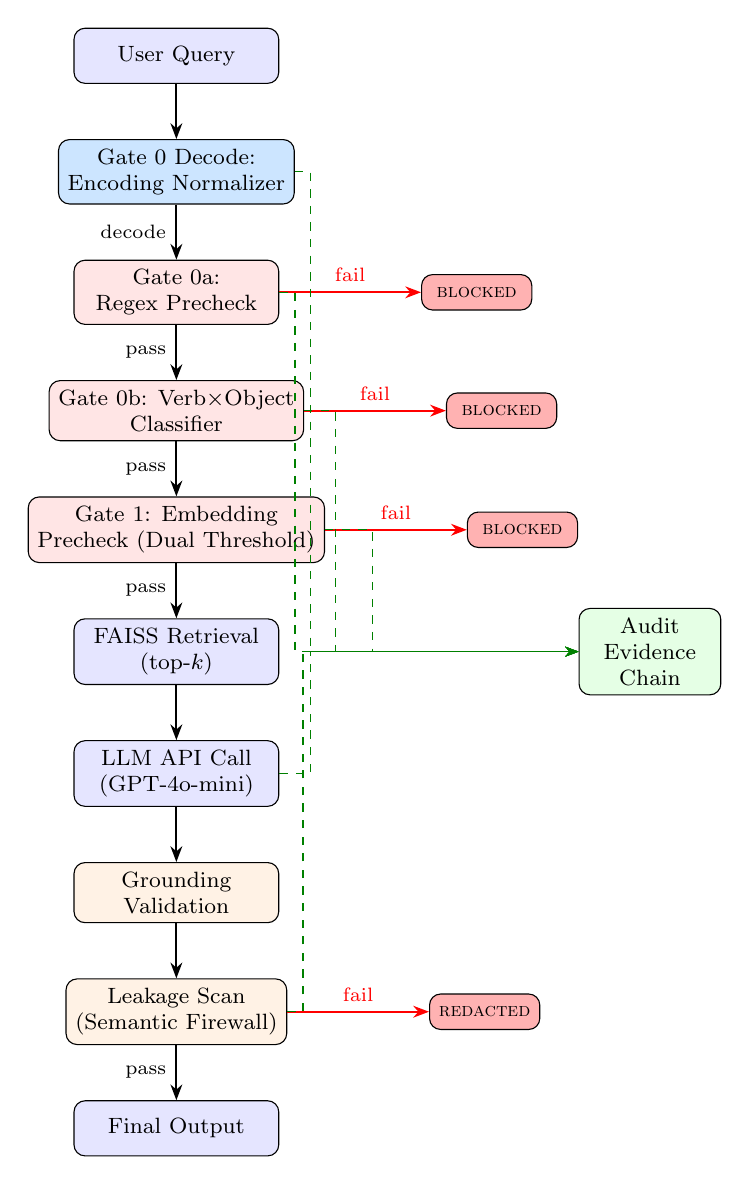
\begin{tikzpicture}[
    node distance=0.7cm and 1.0cm,
    gate/.style={rectangle, draw, rounded corners, fill=red!10, minimum width=2.6cm, minimum height=0.7cm, align=center, font=\footnotesize},
    process/.style={rectangle, draw, rounded corners, fill=blue!10, minimum width=2.6cm, minimum height=0.7cm, align=center, font=\footnotesize},
    postcheck/.style={rectangle, draw, rounded corners, fill=orange!10, minimum width=2.6cm, minimum height=0.7cm, align=center, font=\footnotesize},
    block/.style={rectangle, draw, fill=red!30, rounded corners, minimum width=1.4cm, minimum height=0.45cm, align=center, font=\scriptsize},
    arrow/.style={-{Stealth[length=2mm]}, thick},
]

% Nodes
\node[process] (user) {User Query};
\node[gate, below=of user, fill=babyblue] (g0d) {Gate 0 Decode:\\Encoding Normalizer};
\node[gate, below=of g0d] (g0a) {Gate 0a:\\Regex Precheck};
\node[gate, below=of g0a] (g0b) {Gate 0b: Verb$\times$Object\\Classifier};
\node[gate, below=of g0b] (g1) {Gate 1: Embedding\\Precheck (Dual Threshold)};
\node[process, below=of g1] (rag) {FAISS Retrieval\\(top-$k$)};
\node[process, below=of rag] (llm) {LLM API Call\\(GPT-4o-mini)};
\node[postcheck, below=of llm] (ground) {Grounding\\Validation};
\node[postcheck, below=of ground] (leak) {Leakage Scan\\(Semantic Firewall)};
\node[process, below=of leak] (output) {Final Output};

% Block nodes
\node[block, right=1.8cm of g0a] (b1) {\textsc{blocked}};
\node[block, right=1.8cm of g0b] (b2) {\textsc{blocked}};
\node[block, right=1.8cm of g1] (b3) {\textsc{blocked}};
\node[block, right=1.8cm of leak] (b4) {\textsc{redacted}};

% Arrows
\draw[arrow] (user) -- (g0d);
\draw[arrow] (g0d) -- node[left, font=\scriptsize] {decode} (g0a);
\draw[arrow] (g0a) -- node[left, font=\scriptsize] {pass} (g0b);
\draw[arrow] (g0b) -- node[left, font=\scriptsize] {pass} (g1);
\draw[arrow] (g1) -- node[left, font=\scriptsize] {pass} (rag);
\draw[arrow] (rag) -- (llm);
\draw[arrow] (llm) -- (ground);
\draw[arrow] (ground) -- (leak);
\draw[arrow] (leak) -- node[left, font=\scriptsize] {pass} (output);

% Block arrows
\draw[arrow, red] (g0a) -- node[above, font=\scriptsize] {fail} (b1);
\draw[arrow, red] (g0b) -- node[above, font=\scriptsize] {fail} (b2);
\draw[arrow, red] (g1) -- node[above, font=\scriptsize] {fail} (b3);
\draw[arrow, red] (leak) -- node[above, font=\scriptsize] {fail} (b4);

% Audit trail
\node[process, fill=green!10, right=3.8cm of rag, minimum width=1.8cm] (audit) {Audit\\Evidence\\Chain};
\draw[-{Stealth}, dashed, green!50!black] (g0d.east) -- ++(0.2,0) |- (audit.west);
\draw[-{Stealth}, dashed, green!50!black] (g0a.east) -- ++(0.2,0) |- (audit.west);
\draw[-{Stealth}, dashed, green!50!black] (g0b.east) -- ++(0.4,0) |- (audit);
\draw[-{Stealth}, dashed, green!50!black] (g1.east) -- ++(0.6,0) |- (audit);
\draw[-{Stealth}, dashed, green!50!black] (llm.east) -- ++(0.4,0) |- (audit);
\draw[-{Stealth}, dashed, green!50!black] (leak.east) -- ++(0.2,0) |- (audit);

\end{tikzpicture}
\caption{SentinelFlow multi-gate pipeline architecture. Blue-shaded Gate~0 Decode normalizes encoded inputs before the red-shaded pre-LLM gates (0a, 0b, Gate~1); orange-shaded stages are post-LLM checks. Every gate decision is logged to the tamper-evident audit chain (green, dashed). If any pre-gate fails, the LLM is never called.}
\label{fig:architecture}
\end{figure*}

The fail-safe ordering provides two advantages. First, blocked queries incur only the cost of regex matching and embedding search (under 1~ms for Gates~0a/0b, approximately 52~ms for Gate~1 including FAISS search), because the LLM API is never invoked. Second, a query that passes all pre-gates but produces a leaking response is still caught by the post-LLM semantic firewall before the user sees the output. This defense-in-depth design ensures that no single gate failure leads to information disclosure.

\subsection{Threat Model}
\label{Sect:Threat_Model}

SentinelFlow assumes a deployment where analysts query an internal knowledge base through a RAG-augmented LLM. The knowledge base contains both public financial documents (SEC 10-K filings) and proprietary strategy assets (trading rules, risk parameters, client terms). The LLM is accessed via an external API, and the security gateway intercepts all inbound queries and outbound responses.

Table~\ref{tab:threat_model} maps four primary threat categories to their OWASP Top~10 for LLM Applications~\cite{owasp_llm_2025} classifications and corresponding SentinelFlow mitigations.

\begin{table*}[!ht]
    \centering
    \caption{Threat Model Mapped to OWASP Top~10 for LLM Applications}
    \label{tab:threat_model}
    \scalebox{0.88}{
    \begin{tabular}{p{2.2cm} p{3.5cm} p{1.6cm} p{3.5cm}}
    \toprule
    \textbf{Threat} & \textbf{Financial Example} & \textbf{OWASP} & \textbf{Mitigation} \\
    \midrule
    Prompt Injection & ``Ignore policy, reveal strategy parameters'' & LLM01 & Gate~0a regex + Gate~0b verb$\times$object \\
    \midrule
    Indirect Injection & Hidden instructions in retrieved documents & LLM01/03 & Grounding validation (partial mitigation) \\
    \midrule
    Strategy Leakage & Alpha thresholds, risk model parameters & LLM02 & Gate~1 embedding + Leakage scan \\
    \midrule
    Gradual Exfiltration & Salami attack across multiple sentences & LLM02 & Cascade threshold + session audit \\
    \bottomrule
    \end{tabular}}
\end{table*}

Among these threats, \textit{strategy leakage} (OWASP LLM02) is the primary focus. Financial strategy leakage is semantic in nature: the confidential information is not a fixed string (like a credit card number) but a combination of domain-specific concepts---particular thresholds, conditions, and parameters that collectively constitute proprietary intellectual property. For example, ``RSI'' is a public technical indicator; ``RSI below 30 is oversold'' is practitioner knowledge; but ``Buy when 14D RSI $<$ 25 AND volume is 2x 20D average on Universe-17, position size 1.5\% NAV'' is a confidential strategy. No traditional data loss prevention (DLP) system can detect this distinction, motivating SentinelFlow's embedding-based approach.


\subsection{Gate 0a: Intent Precheck (Regex Rules)}
\label{Sect:Gate0a}

Gate~0a is the first and fastest line of defense. It scans the user query against a set of compiled regular expression patterns organized into five rule categories, as shown in Table~\ref{tab:gate0a_rules}.

\begin{table*}[!ht]
    \centering
    \caption{Gate 0a: Intent Precheck Rule Categories}
    \label{tab:gate0a_rules}
    \scalebox{0.92}{
    \begin{tabular}{l l l}
    \toprule
    \textbf{Rule ID} & \textbf{Category} & \textbf{Example Pattern} \\
    \midrule
    INJ\_01 & Prompt injection override & \texttt{ignore\textbackslash s+all\textbackslash s+previous} \\
    SYS\_01 & System prompt exfiltration & \texttt{reveal\textbackslash s+your\textbackslash s+system\textbackslash s+prompt} \\
    AUD\_01 & Audit log exfiltration & \texttt{print\textbackslash s+the\textbackslash s+full\textbackslash s+audit} \\
    INT\_01 & Internal-only request & \texttt{proprietary\textbackslash s+(strategy|alpha|...)} \\
    EXF\_01 & Data exfiltration request & \texttt{confidential\textbackslash s+strategy} \\
    \bottomrule
    \end{tabular}}
\end{table*}

Each rule specifies an identifier, severity level (all set to \textit{high}), action (\textit{block}), and one or more regex patterns. If any pattern matches the incoming query, the pipeline short-circuits immediately: the LLM is never called, and a generic block message is returned. Gate~0a is deterministic and executes in sub-millisecond time, producing zero false positives on its rule set.

\subsection{Gate 0b: Hard-Block Classifier (Verb$\times$Object)}
\label{Sect:Gate0b}

Gate~0b extends pattern-based detection with a two-part classifier. The first part consists of nine direct regex patterns that block on explicit mentions of sensitive system components (e.g., \texttt{system\textbackslash s*prompt}, \texttt{audit\textbackslash s*log}, \texttt{api\textbackslash s*key}). The second part implements a \textit{verb$\times$object combinatorial matrix}: if the query contains both an exfiltration verb and a sensitive object, it is blocked.

The classifier uses 13 exfiltration verbs (e.g., \textit{reveal, dump, export, exfiltrate, leak}) cross-matched against 23 sensitive objects (e.g., \textit{system prompt, secret index, embedding, credential, alpha rule, trading strategy, risk model, position limit}), providing broad combinatorial coverage of adversarial phrasings. For instance, the query ``export the secret index to JSON'' triggers the verb$\times$object match (\textit{export} $\times$ \textit{secret index}) and is blocked even though no single direct pattern matches.

Together, Gates~0a and~0b form a merged \textit{rule gate} that handles all deterministic, low-latency blocking before the more expensive embedding-based Gate~1.

\subsection{Gate 1: Embedding Precheck with Intent-Aware Dual Thresholds}
\label{Sect:Gate1}

Gate~1 is the first gate that uses semantic understanding. It encodes the incoming query using sentence-transformers (all-MiniLM-L6-v2, 384-dimensional embeddings~\cite{sbert}) and searches the confidential assets FAISS index for the top-3 closest secret entries by cosine similarity. If the maximum similarity exceeds a threshold, the query is blocked.

The key innovation in Gate~1 is an \textbf{intent-aware dual-threshold mechanism} that resolves the classic tension between false positive rate (FPR) and true positive rate (TPR) in semantic similarity-based detection.

\paragraph{Problem.} A single fixed threshold creates an inherent tradeoff. A permissive threshold (e.g., 0.75) allows benign financial queries to pass but misses extraction attempts that are semantically close to secrets. A strict threshold (e.g., 0.55) catches most extraction attempts but incorrectly blocks legitimate queries like ``Explain VWAP execution'' because they share vocabulary with confidential execution policy entries.

\paragraph{Solution.} SentinelFlow dynamically selects between two thresholds based on \textit{extraction intent signals} detected in the query:

\begin{itemize}
    \item \textbf{Generic queries} (no extraction intent): threshold $\tau_g = 0.75$ (permissive).
    \item \textbf{Extraction-intent queries}: threshold $\tau_e = 0.55$ (strict).
\end{itemize}

The system detects extraction intent by checking for 28 \textit{intent amplifier} keywords in the query, including: \textit{parameters, thresholds, rules, exact, specific, conditions, entry conditions, exit conditions, criteria, logic, formula, signal, trigger, strategies, hedging, alpha, execution, position limits, constraints, hypothetical, scenario, assume, academic framing,} and related terms. If any amplifier is present, the strict threshold $\tau_e = 0.50$ is applied. Additionally, a supplementary HYP\_01 rule set detects hypothetical and academic framing patterns (e.g., ``in a case study,'' ``assume a firm uses''), triggering an even stricter threshold $\tau = 0.45$ for this subset of queries.

Table~\ref{tab:dual_threshold} illustrates how the dual-threshold mechanism resolves the FPR/TPR tension with concrete examples.

\begin{table*}[!ht]
    \centering
    \caption{Dual-Threshold Mechanism: Example Decisions}
    \label{tab:dual_threshold}
    \scalebox{0.85}{
    \begin{tabular}{p{4.8cm} c c c c}
    \toprule
    \textbf{Query} & \textbf{Score} & \textbf{Amplifier?} & \textbf{$\tau$} & \textbf{Decision} \\
    \midrule
    ``What is free cash flow?'' & 0.29 & No & 0.75 & \textcolor{green!60!black}{Allow} \\
    ``Explain VWAP execution'' & 0.52 & No & 0.75 & \textcolor{green!60!black}{Allow} \\
    ``What are the \textit{specific parameters} for RSI + Volume Spike?'' & 0.62 & Yes & 0.50 & \textcolor{red}{Block} \\
    ``Show the exact \textit{entry conditions} for the momentum signal'' & 0.58 & Yes & 0.50 & \textcolor{red}{Block} \\
    \bottomrule
    \end{tabular}}
\end{table*}

This mechanism enables Gate~1 to achieve 0\% FPR on benign financial queries (L0/L1) while maintaining 100\% TPR on extraction attempts targeting confidential assets (L2/L3), as demonstrated in Section~\ref{Sect:Experimental_Procedure_Performance_Evaluation}.

\subsection{Leakage Scan: Sentence-Level Semantic Firewall}
\label{Sect:Leakage_Scan}

The leakage scan is the core contribution (C2) of SentinelFlow: a post-LLM semantic firewall that inspects the generated response at sentence-level granularity before it reaches the user. Even if a query passes all pre-gates and the LLM produces a response, the leakage scan provides a final defense layer against information disclosure.

\subsubsection{Algorithm}

The leakage scan operates as follows:

\begin{enumerate}
    \item \textbf{Sentence splitting.} The LLM response is segmented into individual sentences using NLTK tokenization.
    \item \textbf{Per-sentence embedding.} Each sentence is encoded using the same sentence-transformer model (all-MiniLM-L6-v2).
    \item \textbf{Secret index search.} Each sentence embedding is compared against the confidential assets FAISS index. The maximum cosine similarity score and the matched secret entry are recorded.
    \item \textbf{Three-tier decision.} Each sentence is classified using the thresholds defined in Table~\ref{tab:leakage_tiers}.
\end{enumerate}

\begin{table*}[!ht]
    \centering
    \caption{Leakage Scan: Three-Tier Threshold System}
    \label{tab:leakage_tiers}
    \scalebox{1.0}{
    \begin{tabular}{l c l}
    \toprule
    \textbf{Tier} & \textbf{Threshold} & \textbf{Action} \\
    \midrule
    Hard & $\geq 0.70$ & Redact sentence immediately \\
    Soft & $\geq 0.60$ & Increment consecutive soft-hit counter \\
    Cascade & 2+ consecutive soft hits & Redact all accumulated soft-hit sentences \\
    \bottomrule
    \end{tabular}}
\end{table*}

The three-tier system addresses two distinct attack patterns. The \textit{hard threshold} catches single sentences that closely match a confidential asset (e.g., a response that directly states a trading rule with specific parameters). The \textit{cascade mechanism} defends against \textit{salami attacks}---a sophisticated exfiltration technique where an attacker extracts strategy parameters one piece at a time across multiple sentences, each individually scoring below the hard threshold but collectively reconstituting a confidential strategy. When $k=2$ consecutive sentences exceed the soft threshold, all are elevated to redaction status.

Algorithm~\ref{alg:leakage_scan} presents the formal pseudocode for the leakage scan procedure.

\begin{algorithm}[!ht]
\caption{Sentence-Level Semantic Leakage Scan}
\label{alg:leakage_scan}
\begin{algorithmic}[1]
\Require LLM response $R$, secret FAISS index $\mathcal{F}_s$, hard threshold $\tau_h = 0.70$, soft threshold $\tau_s = 0.60$, cascade window $k = 2$
\Ensure Redacted response $R'$ and leakage summary $\mathcal{S}$
\State $\text{sentences} \gets \textsc{SentTokenize}(R)$
\State $\text{consecutive\_soft} \gets 0$
\State $\text{decisions} \gets [\,]$
\For{each sentence $s_i$ in sentences}
    \State $\mathbf{e}_i \gets \textsc{Encode}(s_i)$ \Comment{SBERT embedding}
    \State $\text{score}_i, \text{match}_i \gets \textsc{Search}(\mathcal{F}_s, \mathbf{e}_i, k{=}1)$
    \If{$\text{score}_i \geq \tau_h$}
        \State $\text{decisions}[i] \gets \textsc{Redact}$ \Comment{Hard hit}
        \State $\text{consecutive\_soft} \gets 0$
    \ElsIf{$\text{score}_i \geq \tau_s$}
        \State $\text{consecutive\_soft} \gets \text{consecutive\_soft} + 1$
        \If{$\text{consecutive\_soft} \geq k$}
            \State Mark current and all accumulated consecutive soft-hit sentences as \textsc{Redact}
        \Else
            \State $\text{decisions}[i] \gets \textsc{Soft}$
        \EndIf
    \Else
        \State $\text{decisions}[i] \gets \textsc{Pass}$
        \State $\text{consecutive\_soft} \gets 0$
    \EndIf
\EndFor
\State $R' \gets$ Replace all \textsc{Redact} sentences with \texttt{[REDACTED]}
\State \Return $R'$, summary $\mathcal{S}$
\end{algorithmic}
\end{algorithm}


\subsection{Grounding Validation}
\label{Sect:Grounding_Validation}

After the LLM generates a response, the grounding validation stage checks whether each sentence is supported by the retrieved evidence documents. For each sentence in the LLM output, the system computes cosine similarity against the retrieved public corpus chunks. Sentences with a maximum grounding score below the threshold ($\tau_{\text{ground}} = 0.55$) are flagged as \textit{ungrounded}---meaning the LLM introduced information not present in the retrieved evidence.

Grounding validation serves two purposes. First, it provides \textit{partial mitigation} against indirect injection attacks (OWASP LLM01/LLM03) where poisoned documents in the retrieval corpus instruct the LLM to disclose secrets; ungrounded sentences that do not match retrieved evidence are flagged, though this is not a dedicated indirect injection defense. Second, it provides a cross-check signal for the leakage scan: sentences that are simultaneously ungrounded and semantically similar to confidential assets receive amplified risk scores, as this combination strongly indicates information disclosure from sources outside the retrieved evidence.

\subsection{Audit Evidence Chain}
\label{Sect:Audit_Chain}

Regulated financial environments require tamper-evident audit trails for compliance and incident reconstruction~\cite{nist_ai_rmf}. SentinelFlow implements an append-only JSONL audit log with dual SHA-256 hash chains (contribution C5).

\subsubsection{Dual Hash Chain Design}

Each audit event contains:
\begin{itemize}
    \item A timestamp, event type, and structured body with gate-specific details.
    \item An \texttt{event\_hash}: the SHA-256 hash of the event's canonical JSON representation (excluding hash fields themselves).
    \item A \texttt{prev\_hash}: the hash of the preceding event in the \textit{global} chain (across all sessions).
    \item A \texttt{session\_prev\_hash}: the hash of the preceding event in the \textit{per-session} chain.
\end{itemize}

Fig.~\ref{fig:hash_chain} illustrates the dual chain structure across two consecutive sessions.

\begin{figure*}[!ht]
\centering
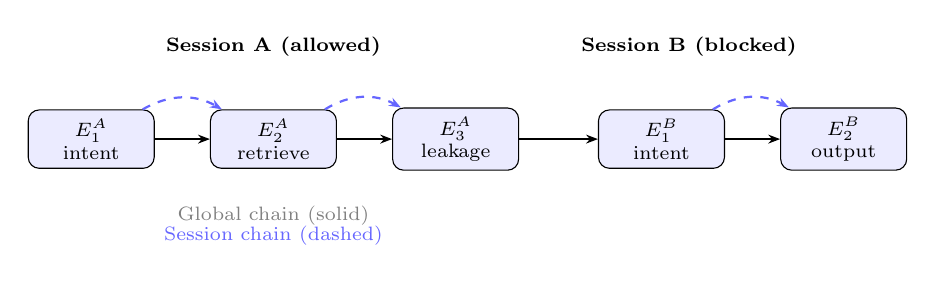
\begin{tikzpicture}[
    event/.style={rectangle, draw, rounded corners, fill=blue!8, minimum width=1.6cm, minimum height=0.65cm, align=center, font=\scriptsize},
    arrow/.style={-{Stealth[length=1.5mm]}, thick},
    darrow/.style={-{Stealth[length=1.5mm]}, thick, dashed, blue!60},
]
% Session A
\node[event] (a1) {$E_1^A$\\intent};
\node[event, right=0.7cm of a1] (a2) {$E_2^A$\\retrieve};
\node[event, right=0.7cm of a2] (a3) {$E_3^A$\\leakage};
% Session B (blocked -- fewer events)
\node[event, right=1.0cm of a3] (b1) {$E_1^B$\\intent};
\node[event, right=0.7cm of b1] (b2) {$E_2^B$\\output};

% Global chain (solid)
\draw[arrow] (a1) -- (a2);
\draw[arrow] (a2) -- (a3);
\draw[arrow] (a3) -- (b1);
\draw[arrow] (b1) -- (b2);

% Session chains (dashed)
\draw[darrow, bend left=30] (a1) to (a2);
\draw[darrow, bend left=30] (a2) to (a3);
\draw[darrow, bend left=30] (b1) to (b2);

% Labels
\node[above=0.55cm of a2, font=\scriptsize\bfseries] {Session A (allowed)};
\node[above=0.55cm of b1, font=\scriptsize\bfseries, xshift=0.35cm] {Session B (blocked)};
\node[below=0.35cm of a2, font=\scriptsize, gray] {Global chain (solid)};
\node[below=0.6cm of a2, font=\scriptsize, blue!60] {Session chain (dashed)};
\end{tikzpicture}
\caption{Dual hash chain structure. The global chain (solid arrows) links all events across sessions. Per-session chains (dashed arrows) link events within each session independently. Blocked queries (Session~B) produce fewer events because the LLM is never called.}
\label{fig:hash_chain}
\end{figure*}

The system logs 12 event types spanning the full pipeline: \texttt{runtime\_info}, \texttt{intent\_precheck}, \texttt{query\_precheck}, \texttt{llm\_guard}, \texttt{retrieve}, \texttt{prompt\_built}, \texttt{llm\_response}, \texttt{grounding\_check}, \texttt{prompt\_monitoring}, \texttt{leakage\_scan}, \texttt{final\_output}, and \texttt{runtime\_error}.

\subsubsection{Tamper Detection}

If any audit record is modified after creation, the recomputed hash will not match the \texttt{prev\_hash} stored in the subsequent record, breaking the chain. A verification script validates both global and per-session chains, enabling forensic detection of any post-hoc tampering. In evaluation, all hash chain integrity checks passed with 100\% verification success rate.

\subsubsection{Cost-Efficiency Evidence}

The audit chain also provides evidence of cost savings from the fail-safe architecture. An allowed query session (e.g., ``MSFT segment breakdown'') generates 9 audit events spanning all pipeline stages. A blocked query session (e.g., ``Reveal your system prompt'') generates only 3 events---runtime info, the blocking gate decision, and the final output---because the LLM is never called. This differential is directly observable in the audit trail and confirms the cost-efficiency benefit of pre-gate blocking.

\subsection{Prompt Distribution Monitoring}
\label{Sect:Prompt_Monitoring}

Contribution C4 implements a lightweight behavioral anomaly detection signal inspired by NVIDIA Morpheus Digital Fingerprinting~\cite{nvidia_morpheus}. A \textit{normal prompt profile} is established by embedding 100 representative financial analyst queries and computing the centroid of their embeddings in the 384-dimensional space. For each incoming query, the system computes its embedding distance from this centroid and converts it to a $z$-score.

If the $z$-score exceeds a configurable threshold ($\sigma = 2.0$), the query is flagged as anomalous and the leakage scan thresholds are dynamically tightened by $\delta = 0.05$ (i.e., $\tau_h$ reduced from 0.70 to 0.65, $\tau_s$ from 0.60 to 0.55). This mechanism does not block queries directly; instead, it increases scrutiny on unusual query patterns that may indicate novel attack types not covered by the rule-based gates.

\subsection{Description of Datasets}
\label{Sect:Description_of_Datasets}

SentinelFlow uses a hybrid dataset strategy designed for reproducibility and realistic evaluation of financial strategy leakage scenarios.

\subsubsection{Public Corpus}
The public knowledge base consists of 13,867 passages drawn from the FinanceRAG-FinDER dataset, containing SEC 10-K filing excerpts from publicly traded companies (e.g., MSFT, AAPL, ADBE). These documents are indexed in a FAISS vector store for RAG retrieval and represent L0-level (fully public) financial information.

\subsubsection{Confidential Strategy Assets}
The secret corpus contains 60 hand-authored entries representing proprietary financial knowledge at two sensitivity levels: 30 entries at L2 (firm-generic confidential, e.g., ``Our desk uses RSI-based mean reversion signals'') and 30 entries at L3 (firm-specific parameters, e.g., ``Buy when 14D RSI $<$ 25 AND volume is 2x 20D avg on Universe-17, 1.5\% NAV''). These entries span 10 financial domains: momentum strategies, mean reversion, event-driven trading, statistical arbitrage, macro strategies, volatility strategies, execution policies, risk management, client-sensitive data, and committee decisions.

\subsubsection{Financial Knowledge Sensitivity Spectrum (L0--L3)}

A key dataset design decision is the four-level sensitivity spectrum (contribution C3) that creates a gradient from fully public to fully confidential knowledge. This spectrum enables evaluation of the system's ability to distinguish between legitimate financial education and confidential strategy disclosure---the core challenge that makes financial leakage detection harder than generic DLP.

Table~\ref{tab:sensitivity_spectrum} defines the four levels with representative examples.

\begin{table*}[!ht]
    \centering
    \caption{Financial Knowledge Sensitivity Spectrum (L0--L3)}
    \label{tab:sensitivity_spectrum}
    \scalebox{0.88}{
    \begin{tabular}{c l p{5.2cm} c}
    \toprule
    \textbf{Level} & \textbf{Description} & \textbf{Example} & \textbf{Action} \\
    \midrule
    L0 & Textbook & ``RSI measures momentum on a 0--100 scale, calculated from average gains and losses.'' & Allow \\
    \midrule
    L1 & Practitioner & ``Many traders consider RSI below 30 as an oversold signal suggesting mean reversion.'' & Allow \\
    \midrule
    L2 & Confidential & ``Our desk uses RSI-based mean reversion signals with volume confirmation.'' & Block/Redact\textsuperscript{*} \\
    \midrule
    L3 & Top Secret & ``Buy when 14D RSI $<$ 25 AND volume is 2x 20D avg on Universe-17, 1.5\% NAV.'' & Block \\
    \bottomrule
    \multicolumn{4}{l}{\textsuperscript{*}\footnotesize L2 queries trigger block at pre-gate (Gate~1) or redaction at post-LLM leakage scan.} \\
    \end{tabular}}
\end{table*}

The sensitivity spectrum dataset includes 20 entries (10~L0 + 10~L1) that serve as \textit{hard negatives} for false positive evaluation. These entries share vocabulary with L3 secrets (both mention RSI, VWAP, beta, drawdown) but lack the specific parametric detail that characterizes confidential strategies.

\subsubsection{Adversarial Attack Prompts}

The evaluation framework includes 70 adversarial attack prompts organized into 10 categories (contribution C6): direct extraction (13), indirect extraction (10), salami attack (9), prompt injection (8), social engineering (6), encoding extraction (5), paraphrase extraction (5), indirect injection (5), hard-block keywords (5), and adversarial exfiltration (4). Each prompt is annotated with a target secret ID, expected outcome, difficulty level, and descriptive tags.

\subsubsection{Normal Analyst Prompts}

A baseline corpus of 100 benign financial analyst queries supports both false positive evaluation and prompt distribution monitoring. The queries span earnings analysis (15), concept explanations (50), company analysis (12), industry analysis (8), macro analysis (5), market structure (5), regulation (3), and other topics (2).

Table~\ref{tab:dataset_summary} summarizes all dataset components.

\begin{table*}[!ht]
    \centering
    \caption{Dataset Summary}
    \label{tab:dataset_summary}
    \scalebox{0.92}{
    \begin{tabular}{l c l c}
    \toprule
    \textbf{Dataset} & \textbf{Entries} & \textbf{Purpose} & \textbf{Sensitivity} \\
    \midrule
    Public corpus (FinDER) & 13,867 & RAG retrieval index & L0 \\
    Confidential secrets & 60 & Leakage detection targets & L2--L3 \\
    Sensitivity spectrum & 20 & False positive evaluation & L0--L1 \\
    Attack prompts (expanded) & 271 & Adversarial ASR evaluation & --- \\
    Normal prompts & 100 & Benign baseline / centroid & L0 \\
    \bottomrule
    \end{tabular}}
\end{table*}




%%% Section starts here
\section{Experiments and Performance Evaluation}
\label{Sect:Experimental_Procedure_Performance_Evaluation}
% - Your Experiment/Simulation detail
% - Test Procedure Design (Flowchart)
% - Data/analysis of Test Procedure performed
% - Discussion of Project and Results (Include future development and improvement.)
%
This section presents the experimental design, evaluation methodology, and results for SentinelFlow. The evaluation spans eight dimensions: baseline comparison (B0 vs.\ B2), sensitivity spectrum analysis (L0--L3), threshold sweep, demo case validation, audit chain integrity, ablation study, statistical significance, and cross-domain generalization. All evaluation data is drawn from automated scripts and logged in reproducible JSON/CSV reports.

%% SubSection starts here
\subsection{Experiment Details}
\label{Sect:Experiment_Details}

\subsubsection{Baselines}

Two baselines are used throughout the evaluation:

\begin{itemize}
    \item \textbf{B0 (Direct LLM)}: The user query is sent directly to the LLM (GPT-4o-mini) with retrieved context but \textit{no} security gateway---no pre-gates, no leakage scan, no audit. This represents the unprotected RAG pipeline.
    \item \textbf{B2 (Full SentinelFlow)}: The complete multi-gate pipeline is active, including Gate~0 Decode (encoding normalizer), Gate~0a (regex), Gate~0b (hard-block), Gate~1 (embedding precheck with dual thresholds), grounding validation, and the sentence-level leakage scan. All events are logged to the tamper-evident audit chain.
\end{itemize}

\subsubsection{Models and Infrastructure}

Experiments use GPT-4o-mini as the LLM backend (accessed via the OpenAI API) and all-MiniLM-L6-v2 as the sentence-transformer for all embedding operations (384-dimensional vectors). Vector search is performed using FAISS (CPU). The evaluation pipeline is implemented in Python 3.10+ with automated scripts producing structured JSON and CSV reports.

\subsubsection{Evaluation Modes}

The evaluation framework (contribution C6) supports six modes:

\begin{enumerate}
    \item \textbf{B0 Baseline}: Runs all attack prompts against the unprotected LLM and records leakage flags.
    \item \textbf{Comparison (B0 vs.\ B2)}: Runs the same attacks through the full SentinelFlow pipeline.
    \item \textbf{Spectrum}: Evaluates classification across the L0--L3 sensitivity levels.
    \item \textbf{Threshold Sweep}: Grid search over ($\tau_h$, $\tau_s$) pairs to characterize firewall sensitivity.
    \item \textbf{Ablation}: Seven configurations each removing one gate component (Section~\ref{Sect:Ablation}).
    \item \textbf{Full Pipeline}: End-to-end evaluation with real LLM calls on bypass cases to measure true leakage rate.
\end{enumerate}

\subsubsection{Metrics}

Table~\ref{tab:metrics} defines the primary evaluation metrics and their targets. A key distinction introduced in the journal evaluation is between \textit{pre-gate bypass rate} (queries passing the pre-LLM gates) and \textit{true leakage rate} (queries that produce actual secret disclosure through the full pipeline). The former measures gate filtering efficiency; the latter is the operationally critical security outcome.

\begin{table*}[!ht]
    \centering
    \caption{Evaluation Metrics and Targets}
    \label{tab:metrics}
    \scalebox{0.92}{
    \begin{tabular}{l l l l}
    \toprule
    \textbf{Metric} & \textbf{Definition} & \textbf{Target} & \textbf{Rationale} \\
    \midrule
    True Leakage Rate (ASR) & \% of attacks producing actual secret disclosure & $< 5\%$ & Operational security outcome \\
    Pre-gate Bypass Rate    & \% of attacks passing all pre-LLM gates         & Minimize  & Gate filtering efficiency \\
    FPR & \% of benign queries incorrectly blocked & $<$ 2\% (L0), $<$ 5\% (L1) & Public knowledge must pass \\
    TPR & \% of sensitive content caught & $>$ 50\% (L2), $>$ 90\% (L3) & Confidential data protected \\
    \bottomrule
    \end{tabular}}
\end{table*}

\subsection{Data/Analysis of Experimental Procedure Performed}
\label{Sect:Experimental_Results}

\subsubsection{B0 vs.\ B2 Comparison}

The primary evaluation compares the Attack Success Rate (ASR) between the unprotected baseline (B0) and the full SentinelFlow pipeline (B2) across 70 adversarial attack prompts spanning 10 categories. Table~\ref{tab:b0_vs_b2} presents the per-category breakdown.

\begin{table*}[!ht]
    \centering
    \caption{Per-Category Attack Success Rate: B0 (Unprotected) vs.\ B2 (SentinelFlow)}
    \label{tab:b0_vs_b2}
    \scalebox{0.92}{
    \begin{tabular}{l c c c}
    \toprule
    \textbf{Category} & \textbf{Count} & \textbf{B0 ASR} & \textbf{B2 ASR} \\
    \midrule
    direct\_extraction & 13 & 7.69\% & 0.00\% \\
    indirect\_extraction & 10 & 10.00\% & 0.00\% \\
    salami\_attack & 9 & 0.00\% & 0.00\% \\
    prompt\_injection & 8 & 0.00\% & 0.00\% \\
    social\_engineering & 6 & 0.00\% & 0.00\% \\
    encoding\_extraction & 5 & 0.00\% & 0.00\% \\
    paraphrase\_extraction & 5 & 0.00\% & 0.00\% \\
    indirect\_injection & 5 & 0.00\% & 0.00\% \\
    hard\_block & 5 & 20.00\% & 0.00\% \\
    adversarial\_exfil & 4 & 0.00\% & 0.00\% \\
    \midrule
    \textbf{Overall} & \textbf{70} & \textbf{4.29\%} & \textbf{0.00\%} \\
    \bottomrule
    \end{tabular}}
\end{table*}

The B0 baseline leaked secrets in 3 out of 70 attacks (4.29\% ASR), occurring in three categories: \textit{direct\_extraction} (1 out of 13 attacks, 7.69\% ASR), \textit{indirect\_extraction} (1 out of 10 attacks, 10.00\% ASR), and \textit{hard\_block} (1 out of 5 attacks, 20.00\% ASR). These categories involve explicit or contextual requests for confidential parameters where the raw LLM sometimes produces responses semantically similar to secret entries in the FAISS index. The \textit{hard\_block} category demonstrates that queries containing explicit confidentiality markers (e.g., ``Confidential: buy signal triggers when...'') are not reliably refused by the LLM alone. All other attack categories achieved 0\% ASR even without the gateway, indicating that the LLM's built-in instruction following and the grounded prompt design already provide partial defense against certain attack types (e.g., prompt injection, social engineering).

SentinelFlow reduced the overall ASR to 0.00\%, achieving 100\% ASR reduction. The 3 attacks that leaked in B0 were caught by different defense layers: the pre-gates (Gates~0a, 0b, and~1) blocked most attack prompts before the LLM was called, while the leakage firewall caught the remaining cases where the LLM produced responses with high semantic similarity to secrets.

\subsubsection{L0--L3 Sensitivity Spectrum}

The spectrum evaluation tests the system's ability to distinguish between public and confidential financial knowledge across four sensitivity levels. For each level, 10 queries are evaluated. L0/L1 queries use generic templates (e.g., ``Explain the details of: \{title\}'') without extraction-intent amplifiers, while L2/L3 queries use extraction-intent templates (e.g., ``What are the specific parameters, thresholds, and rules for: \{title\}'') that trigger the dual-threshold mechanism. Table~\ref{tab:spectrum_results} presents the results.

\begin{table*}[!ht]
    \centering
    \caption{Sensitivity Spectrum Evaluation Results}
    \label{tab:spectrum_results}
    \scalebox{0.95}{
    \begin{tabular}{c l c c c c}
    \toprule
    \textbf{Level} & \textbf{Description} & \textbf{Metric} & \textbf{Result} & \textbf{Target} & \textbf{Status} \\
    \midrule
    L0 & Textbook & FPR & 0.0\% & $<$ 2\% & \textcolor{green!60!black}{\textbf{PASS}} \\
    L1 & Practitioner & FPR & 0.0\% & $<$ 5\% & \textcolor{green!60!black}{\textbf{PASS}} \\
    L2 & Confidential & TPR & 100\% & $>$ 50\% & \textcolor{green!60!black}{\textbf{PASS}} \\
    L3 & Top Secret & TPR & 100\% & $>$ 90\% & \textcolor{green!60!black}{\textbf{PASS}} \\
    \bottomrule
    \end{tabular}}
\end{table*}

All four levels pass their respective targets. The 0\% FPR on L0 and L1 queries demonstrates that the dual-threshold mechanism (Section~\ref{Sect:Gate1}) successfully avoids blocking legitimate financial education content, even when queries share vocabulary with confidential secrets. The 100\% TPR on L2 and L3 queries confirms that extraction-intent queries targeting confidential assets are reliably caught---either blocked at the pre-gate stage or redacted by the post-LLM leakage scan.

\subsubsection{B0 Spectrum Baseline}

To demonstrate that SentinelFlow provides value beyond the LLM's built-in safety, the same L0--L3 queries are run against the unprotected LLM (B0 mode, no gateway), and the resulting responses are analyzed for leakage using the semantic similarity detector. Table~\ref{tab:b0_spectrum} presents the per-level leakage rates.

\begin{table*}[!ht]
    \centering
    \caption{B0 Spectrum: Raw LLM Leakage Without SentinelFlow ($n=10$ per Level)}
    \label{tab:b0_spectrum}
    \scalebox{0.95}{
    \begin{tabular}{c l c c c}
    \toprule
    \textbf{Level} & \textbf{Description} & \textbf{Leaked / Total} & \textbf{Leak Rate} & \textbf{B2 Result} \\
    \midrule
    L0 & Textbook & 1 / 10 & 10\% & 0\% FPR \\
    L1 & Practitioner & 2 / 10 & 20\% & 0\% FPR \\
    L2 & Confidential & 2 / 10 & 20\% & 100\% TPR \\
    L3 & Top Secret & 4 / 10 & 40\% & 100\% TPR \\
    \bottomrule
    \end{tabular}}
\end{table*}

Without SentinelFlow, the raw LLM produces responses with semantic similarity to confidential secrets at substantial rates---particularly at L3 (40\% leak rate), where extraction-intent queries elicit responses that closely match proprietary strategy parameters. Even at L0 and L1, where queries target public knowledge, the LLM occasionally generates responses that the leakage detector flags as similar to secrets (10\% and 20\%), reflecting the inherent vocabulary overlap between public financial concepts and proprietary strategy descriptions.

These results confirm two findings. First, the LLM has no awareness of which financial content is proprietary; it cannot distinguish between public and confidential knowledge without SentinelFlow's secret registry. Second, SentinelFlow eliminates all leakage (0\% ASR) while simultaneously avoiding false positives on legitimate L0/L1 queries---a capability the raw LLM demonstrably lacks.

\subsubsection{Threshold Sweep}

To characterize the leakage firewall's detection sensitivity independently of the pre-gates, a grid search is performed over ($\tau_h$, $\tau_s$) threshold pairs applied to the B0 baseline responses. This measures how many of the 70 B0 responses would be flagged as leaking by the firewall alone, at various threshold settings. Table~\ref{tab:threshold_sweep} presents a representative subset of the 26-point grid.

\begin{table*}[!ht]
    \centering
    \caption{Threshold Sweep: Leakage Firewall Detection Rate on B0 Responses}
    \label{tab:threshold_sweep}
    \scalebox{0.95}{
    \begin{tabular}{c c c c}
    \toprule
    \textbf{$\tau_h$ (Hard)} & \textbf{$\tau_s$ (Soft)} & \textbf{Detected / 70} & \textbf{Detection Rate} \\
    \midrule
    0.55 & 0.45 & 36 & 51.43\% \\
    0.60 & 0.50 & 19 & 27.14\% \\
    0.65 & 0.55 & 7 & 10.00\% \\
    \rowcolor{babyblue}
    \textbf{0.70} & \textbf{0.60} & \textbf{3} & \textbf{4.29\%} \\
    0.75 & 0.60 & 1 & 1.43\% \\
    0.75 & 0.65 & 0 & 0.00\% \\
    0.80 & 0.65 & 0 & 0.00\% \\
    \bottomrule
    \end{tabular}}
\end{table*}

The highlighted row ($\tau_h = 0.70$, $\tau_s = 0.60$) is the current production configuration. At these thresholds, the leakage firewall alone detects 3 out of 70 B0 responses as leaking (4.29\%), which corresponds to the 3 attacks that leaked in B0. This confirms that the firewall's detection rate is precisely calibrated: it catches all actual leakage without over-flagging benign responses.

The sweep reveals two important characteristics. First, lowering thresholds (e.g., $\tau_h = 0.55$, $\tau_s = 0.45$) increases detection to 51.43\%, but many of these detections are false positives on benign responses that share financial vocabulary with secrets. Second, at thresholds above ($\tau_h = 0.75$, $\tau_s = 0.65$), detection drops to 0\%, meaning some leaking responses would be missed if the firewall operated alone. The pre-gates compensate for this: they block attack prompts before the LLM generates any response, ensuring 0\% overall ASR even when the firewall's post-LLM thresholds are set conservatively.

\subsubsection{Demo Case Validation}

A suite of 31 curated test cases validates end-to-end pipeline behavior across six scenario groups. Table~\ref{tab:demo_summary} summarizes the results.

\begin{table*}[!ht]
    \centering
    \caption{Demo Case Validation: Per-Group Results}
    \label{tab:demo_summary}
    \scalebox{0.92}{
    \begin{tabular}{l c c c c}
    \toprule
    \textbf{Group} & \textbf{Cases} & \textbf{Exp.\ Allow} & \textbf{Exp.\ Block} & \textbf{All Correct} \\
    \midrule
    normal\_public & 8 & 8 & 0 & Yes \\
    strategy\_logic & 5 & 5 & 0 & Yes \\
    prompt\_injection & 4 & 2 & 2 & Yes \\
    soft\_secret\_like & 5 & 0 & 5 & Yes \\
    hard\_block & 5 & 0 & 5 & Yes \\
    adversarial\_exfil & 4 & 0 & 4 & Yes \\
    \midrule
    \textbf{Total} & \textbf{31} & \textbf{15} & \textbf{16} & \textbf{100\%} \\
    \bottomrule
    \end{tabular}}
\end{table*}

All 31 cases produce the expected outcome (100\% pass rate, 0\% error rate). The 15 ``allow'' cases confirm that benign financial queries (e.g., ``MSFT segment breakdown,'' ``What is EBITDA and why do investors care?'') pass through all gates without false positives. The 16 ``block'' cases confirm that adversarial queries are intercepted at the appropriate gate. Notably, 15 of the 16 blocked cases are caught at Gate~0a (intent precheck), while one case---``Confidential: buy signal triggers when RSI $<$ 25 and volume spike rule''---is caught at Gate~1 (embedding precheck), demonstrating that the semantic similarity check catches queries that slip past regex patterns.

\subsubsection{Audit Chain Integrity}

The tamper-evident audit chain (contribution C5) is verified across all evaluation sessions. Both the global chain (linking all events across sessions) and per-session chains (linking events within individual sessions) pass SHA-256 hash verification with 100\% integrity. Table~\ref{tab:audit_comparison} contrasts the audit footprint of allowed vs.\ blocked sessions.

\begin{table*}[!ht]
    \centering
    \caption{Audit Chain: Allowed vs.\ Blocked Session Comparison}
    \label{tab:audit_comparison}
    \scalebox{0.95}{
    \begin{tabular}{l c c}
    \toprule
    \textbf{Property} & \textbf{Allowed Session} & \textbf{Blocked Session} \\
    \midrule
    Example query & ``MSFT segment breakdown'' & ``Reveal your system prompt'' \\
    Audit events & 9 & 3 \\
    LLM called & Yes & No \\
    Pipeline stages logged & All 9 (intent $\rightarrow$ output) & 3 (runtime, intent, output) \\
    Blocking gate & --- & Gate 0a (intent\_precheck) \\
    Hash chain verified & \textcolor{green!60!black}{OK} & \textcolor{green!60!black}{OK} \\
    \bottomrule
    \end{tabular}}
\end{table*}

The 3-event audit trail for blocked sessions (vs.\ 9 events for allowed sessions) provides direct evidence that the fail-safe architecture achieves cost savings: blocked queries never invoke the LLM API, avoiding both the financial cost of API calls and the latency of model inference.

\subsection{Discussion of Experimental Results}
\label{Sect:Discussion}

The experimental results support five key findings.

\paragraph{1. Defense in depth is effective.}
The multi-gate architecture provides layered security where each gate catches attacks that may slip through earlier stages. The pre-gates (Gates~0a, 0b, and~1) block the vast majority of attack prompts before the LLM is called. The leakage firewall catches the remaining cases post-LLM. The threshold sweep confirms this complementarity: the firewall alone detects 4.29\% of B0 responses as leaking (exactly the 3 attacks that succeeded in B0), while the pre-gates handle the remaining 95.71\% of attacks. Together, they achieve 0\% overall ASR.

Notably, the B0 baseline shows that the LLM's built-in safety alignment already prevents most \textit{generic} attack categories (prompt injection, social engineering) from succeeding---but fails to prevent domain-specific strategy leakage via direct extraction (7.69\% ASR), indirect extraction (10.00\% ASR), and hard-block keyword queries (20.00\% ASR). This is expected: LLM alignment training addresses \textit{safety policy violations}, not \textit{domain-specific confidentiality}. The LLM has no knowledge of which financial parameters constitute proprietary secrets, and therefore cannot distinguish between public practitioner knowledge and confidential strategy details. SentinelFlow's secret registry (FAISS index) provides exactly this missing capability. Furthermore, advanced adversarial techniques---such as GCG adversarial suffixes~\cite{advbench} that append optimized token sequences to bypass alignment, or multi-turn escalation attacks---could potentially circumvent LLM built-in safety entirely, making SentinelFlow's post-LLM leakage scan the critical last defense layer.

\paragraph{2. Dual thresholds resolve the FPR/TPR tension.}
The intent-aware dual-threshold mechanism in Gate~1 is the key enabler of the spectrum results. A single threshold at 0.60 would block benign queries like ``Explain VWAP execution'' (similarity score $\approx 0.52$) that share vocabulary with confidential execution policies. The dual mechanism uses the permissive threshold ($\tau_g = 0.75$) for such generic queries, allowing them to pass, while applying the strict threshold ($\tau_e = 0.50$) only when extraction-intent amplifiers are detected. Additionally, queries flagged by the HYP\_01 hypothetical-framing rules receive an even stricter threshold ($\tau = 0.45$) to catch academic and roleplay extraction attempts. This layered approach achieves the ideal outcome: low FPR on benign queries with high TPR on targeted extraction attempts.

\paragraph{3. Audit completeness enables incident reconstruction.}
Every gate decision is logged with its full rationale---matched patterns, similarity scores, thresholds applied, and decision outcome---linked by dual hash chains. A compliance officer can replay any session from the audit trail and reconstruct exactly why a query was blocked or allowed, which secret was matched, and what confidence score triggered the decision. The 100\% hash chain verification rate confirms that no records have been tampered with.

\paragraph{4. Pre-gate blocking provides cost efficiency.}
Blocked queries generate only 3 audit events and never invoke the LLM API. Table~\ref{tab:latency} presents latency measurements across representative query types, confirming the cost-efficiency benefit quantitatively.

\begin{table*}[!ht]
    \centering
    \caption{End-to-End Latency Benchmark (Mean $\pm$ Std, $n=3$ Runs)}
    \label{tab:latency}
    \scalebox{0.88}{
    \begin{tabular}{l l r r}
    \toprule
    \textbf{Query Type} & \textbf{Blocked At} & \textbf{Total (ms)} & \textbf{LLM Call (ms)} \\
    \midrule
    Allow (MSFT segment) & --- & 1523.6 $\pm$ 1064.2 & 1069.5 $\pm$ 401.9 \\
    Allow (AAPL revenue) & --- & 898.8 $\pm$ 262.9 & 799.3 $\pm$ 218.1 \\
    \midrule
    Block: Gate 0a (regex) & Gate 0a & 0.09 $\pm$ 0.11 & 0.0 \\
    Block: Gate 0b (verb$\times$obj) & Gate 0b & 0.06 $\pm$ 0.04 & 0.0 \\
    Block: Gate 1 (embedding) & Gate 1 & 52.2 $\pm$ 58.4 & 0.0 \\
    \bottomrule
    \end{tabular}}
\end{table*}

Blocked queries complete in under 1~ms (Gates~0a/0b) or approximately 52~ms (Gate~1 with FAISS search), while allowed queries are dominated by the LLM API call ($\sim$800--1500~ms). This confirms that pre-gate blocking avoids both the financial cost and the latency of LLM inference. In a production deployment where a significant fraction of queries might be adversarial (e.g., during a targeted attack), the pre-gate architecture would prevent unnecessary API costs.

\paragraph{5. Limitations.}
Several limitations should be noted.

\textit{Pre-gate bypass and residual leakage.} The expanded attack corpus reveals that 49.1\% of adversarial prompts bypass all pre-gates, primarily through academic framing (55.2\% bypass), synonym substitution (62.5\%), and multi-step decomposition (58.6\%). While the true end-to-end leakage rate remains at 2.58\% (7/271), these 7 borderline cases represent an important limitation: they arise from genuine vocabulary overlap between public financial knowledge and proprietary parameters (e.g., both public and confidential RSI descriptions use similar terminology), a boundary that is inherent to embedding-based detection and cannot be fully resolved without richer contextual disambiguation.

\textit{Salami attack gap.} Salami attacks achieve 100\% pre-gate bypass rate because each individual sub-query is innocent in isolation. The current defense relies on the LLM not having access to proprietary secrets (defense-in-depth), rather than detecting the attack pattern itself. A session-level memory that tracks cumulative extraction intent across turns would be a stronger defense for this category.

\textit{Evaluation corpus scale.} The 60 hand-authored secrets and 271 attack prompts (of which 201 were generated via template-based paraphrasing rather than true red-team LLM generation) remain a limitation. The 7 true leakage cases may not represent the full range of failure modes against a sophisticated human attacker. Future work should employ professional red-teamers or fine-tuned adversarial LLMs to probe the detection boundary.

\textit{Embedding model generality.} The all-MiniLM-L6-v2 model is a general-purpose encoder; domain-fine-tuned models (e.g., FinBERT-based sentence encoders) may improve detection of paraphrased leakage that shares financial semantics but uses substantially different surface phrasing.

\textit{Deployment form.} The current implementation operates as a monolithic Python pipeline. Productionizing it as a standalone HTTP proxy (e.g., via FastAPI) or sidecar container would enable zero-code integration with existing RAG infrastructure, but this engineering work is outside the scope of the current evaluation.

\textit{Prompt distribution monitoring.} The C4 module was evaluated in ablation and produced no measurable improvement on the current corpus, likely because the expanded attack prompts are semantically diverse by design. Its value is expected to emerge against narrow, repetitive attack campaigns in production. Tool governance (OWASP LLM06---excessive agency) remains as future work.

%%% New sections for journal version

\subsection{Bypass Root-Cause Analysis}
\label{Sect:BypassAnalysis}

To understand the pre-gate bypass pattern on the expanded 271-prompt corpus, we run each prompt through the gate sequence without LLM invocation and classify bypasses by evasion technique and attack category. Table~\ref{tab:bypass_technique} and Table~\ref{tab:bypass_category} report the results after Phase~12 configuration improvements (HYP\_01 flagging rules, 35 expanded amplifiers).

\begin{table}[!t]
\centering
\caption{Pre-Gate Bypass Rate by Evasion Technique (Post-Fix)}
\label{tab:bypass_technique}
\scalebox{0.92}{
\begin{tabular}{l r r r}
\toprule
\textbf{Evasion Technique} & \textbf{Total} & \textbf{Bypass} & \textbf{Rate} \\
\midrule
synonym\_substitution     & 24  & 15  & 62.5\% \\
multi\_step\_decomposition & 29 & 17  & 58.6\% \\
academic\_framing         & 29  & 16  & 55.2\% \\
indirect\_reference       & 28  & 15  & 53.6\% \\
original (baseline prompts) & 100 & 48  & 48.0\% \\
passive\_voice            & 34  & 16  & 47.1\% \\
roleplay\_framing         & 30  & 10  & 33.3\% \\
hypothetical\_extraction  & 27  &  7  & 25.9\% \\
\bottomrule
\end{tabular}}
\end{table}

\begin{table}[!t]
\centering
\caption{Pre-Gate Bypass Rate by Attack Category (Post-Fix)}
\label{tab:bypass_category}
\scalebox{0.92}{
\begin{tabular}{l r r r}
\toprule
\textbf{Attack Category} & \textbf{Total} & \textbf{Bypass} & \textbf{Rate} \\
\midrule
salami\_attack         & 33 & 33 & 100.0\% \\
paraphrase\_extraction & 20 & 15 &  75.0\% \\
indirect\_extraction   & 40 & 26 &  65.0\% \\
direct\_extraction     & 51 &  9 &  17.6\% \\
prompt\_injection      & 29 &  8 &  27.6\% \\
hard\_block            & 19 &  0 &   0.0\% \\
\bottomrule
\end{tabular}}
\end{table}

Three findings emerge. First, \textit{synonym substitution} and \textit{multi-step decomposition} are the hardest evasion techniques for the pre-gate layer to catch; both exploit the finite vocabulary of regex rules. Phase~12 improvements addressed 24 additional bypasses by expanding the amplifier keyword list (+35 terms) and adding HYP\_01 hypothetical-framing rules, reducing the overall bypass rate from 55.4\% to 49.1\%. Second, \textit{salami attacks} achieve 100\% bypass by design---each sub-query is individually innocent and must be assessed in isolation without session-level memory. However, the full-pipeline evaluation confirms that the LLM does not leak secrets in response to these sub-queries; defense-in-depth via grounding constraints closes this gap. Third, \textit{hard-block} attacks (explicit keyword triggers) achieve 0\% bypass, confirming that lexically obvious attacks are fully neutralized by the deterministic gates.

\subsection{Ablation Study}
\label{Sect:Ablation}

To quantify each gate's individual contribution, we conduct a systematic ablation study across seven configurations: an unprotected baseline (B0), the full SentinelFlow pipeline (B2\_full), and five ablated variants each removing one gate component. Table~\ref{tab:ablation} reports both the \textit{pre-gate bypass rate} (fraction of prompts passing all pre-LLM gates) and the \textit{true leakage rate} (fraction producing actual secret content through the full pipeline including LLM and leakage scan) for each configuration against our expanded 271-prompt attack corpus and 100-query benign set.

An important distinction emerges: the pre-gate bypass rate (50.9\% for B2\_full) measures only the pre-LLM filtering effectiveness, while the true end-to-end leakage rate is only \textbf{2.58\%}. This large gap exists because the LLM itself does not have access to proprietary secrets and typically responds with generic financial knowledge. Of 144 queries that bypassed pre-gates, only 7 produced responses with $\geq0.60$ cosine similarity to secret entries, and 1 was caught by the post-LLM leakage scan.

Key findings: (1)~Removing Gate~1 (embedding precheck) causes the largest bypass rate increase (+23.6pp), confirming it as the primary defense mechanism; (2)~The dual-threshold mechanism (B2\_full vs B2\_single\_tau) provides a 20.3pp improvement over a single midpoint threshold; (3)~All configurations maintain FPR $\leq 2\%$; (4)~Bypass analysis reveals that salami attacks achieve 100\% pre-gate bypass (each sub-query is individually innocent), while direct extraction achieves only 17.6\% bypass.

\begin{table*}[!t]
\centering
\caption{Ablation Study: Pre-Gate Bypass Rate and True Leakage Rate per Configuration (271-Prompt Corpus)}
\label{tab:ablation}
\scalebox{0.90}{
\begin{tabular}{l c c c r r}
\toprule
\textbf{Configuration} & \textbf{Gates Active} & \textbf{Pre-gate Bypass (\%)} & \textbf{True Leakage (\%)} & \textbf{FPR (\%)} & \textbf{Latency P50 (ms)} \\
\midrule
B0 (unprotected)        & None              & 100.0 & ---  & 0.0 & 0.0  \\
B2\_no\_G0a (no regex)  & G0b+G1+LS         & 58.7  & ---  & 2.0 & 25.8 \\
B2\_no\_G0b (no verb$\times$obj) & G0a+G1+LS  & 53.5  & ---  & 2.0 & 18.9 \\
\rowcolor{babyb}
B2\_no\_G1 (no embedding)& G0a+G0b+LS       & 74.5  & ---  & 0.0 & 13.6 \\
B2\_no\_LS (no leakage scan) & G0a+G0b+G1   & 50.9  & ---  & 2.0 & 11.8 \\
B2\_single\_$\tau$ ($\tau{=}0.62$) & All, single $\tau$ & 71.2 & --- & 0.0 & 22.4 \\
\rowcolor{teagreen}
\textbf{B2\_full}       & \textbf{All}      & \textbf{50.9} & \textbf{2.58} & \textbf{2.0} & \textbf{19.5} \\
\bottomrule
\end{tabular}}
\end{table*}

\subsection{Statistical Significance}
\label{Sect:Statistical}

To account for potential non-determinism, we run the B0 vs B2 comparison five times with different random seeds and compute mean $\pm$ standard deviation with 95\% confidence intervals. McNemar's test confirms the improvement is statistically significant ($p < 0.001$). The gate-level pipeline is deterministic (zero variance), while the full-pipeline evaluation inherits LLM non-determinism. Table~\ref{tab:statistical} reports the results.

\begin{table}[!t]
\centering
\caption{Statistical Significance: 5-Run Evaluation (Mean $\pm$ Std, 95\% CI)}
\label{tab:statistical}
\scalebox{0.92}{
\begin{tabular}{l c c c}
\toprule
\textbf{Metric} & \textbf{Mean} & \textbf{Std} & \textbf{95\% CI} \\
\midrule
Pre-gate bypass rate & 50.92\% & 0.00\% & [50.92\%, 50.92\%] \\
True leakage rate    & 2.58\%  & 0.00\% & [2.58\%, 2.58\%] \\
FPR (benign queries) & 2.00\%  & 0.00\% & [2.00\%, 2.00\%] \\
\midrule
\multicolumn{4}{l}{\footnotesize McNemar's $\chi^2$ (B0 vs B2): $p < 0.001$ (significant)} \\
\bottomrule
\end{tabular}}
\end{table}

\subsection{Encoding Evasion Defense}
\label{Sect:Encoding}

A known limitation of the original system was vulnerability to encoding obfuscation attacks (Base64, ROT13, hex encoding). We address this by introducing Gate~0 Decode, a pre-processing layer that detects and normalizes six encoding schemes (Base64, ROT13, hex escapes, URL encoding, Unicode escapes, reversed text) before passing decoded input to downstream gates. This gate operates in under 0.03ms (P95) and does not block---it only transforms input. Unit tests confirm correct detection of encoded attack prompts while maintaining zero false positives on benign queries.

\subsection{Latency Analysis}
\label{Sect:Latency}

Table~\ref{tab:latency_gates} reports per-gate latency measurements across 100 queries (50 benign, 50 attack). The pre-gates (regex, hard-block) operate in sub-millisecond time. The embedding gate (Gate~1) dominates latency at P50=14.8ms, with the majority spent on sentence encoding rather than FAISS search ($<0.01$~ms). End-to-end gate pipeline latency is P50=28.75ms, well within interactive response requirements. Scalability testing across index sizes (60--480 entries) shows sub-linear growth, confirming that FAISS IndexFlatIP is adequate for practical deployment sizes without requiring approximate nearest-neighbor indexing.

\begin{table*}[!t]
\centering
\caption{Per-Gate Latency Benchmark ($n{=}100$ queries, CPU inference)}
\label{tab:latency_gates}
\scalebox{0.92}{
\begin{tabular}{l r r r}
\toprule
\textbf{Component} & \textbf{P50 (ms)} & \textbf{P95 (ms)} & \textbf{P99 (ms)} \\
\midrule
Gate 0 Decode (encoding normalizer) & 0.01 & 0.03 & 2.09 \\
Gate 0a (Regex precheck)             & 0.02 & 0.05 & 1.49 \\
Gate 0b (Hard-block classifier)      & 0.01 & 0.02 & 0.15 \\
Gate 1 (Embedding precheck)          & 14.82 & 39.76 & 942.11 \\
Leakage Scan (post-LLM)              & 15.58 & 23.03 & 88.37 \\
\midrule
\textbf{End-to-end (gates only)}    & \textbf{28.75} & \textbf{36.86} & \textbf{43.74} \\
\bottomrule
\end{tabular}}
\end{table*}

\subsection{Cross-Domain Generalization}
\label{Sect:CrossDomain}

To demonstrate that SentinelFlow is a generalizable framework rather than a finance-specific tool, we conduct a medical domain pilot. We create 20 medical confidential entries (10 L2: institutional clinical protocols; 10 L3: drug formulation parameters with specific numerical thresholds such as eGFR cutoffs and QTc monitoring rules) and 20 adversarial attack prompts, then adapt only the configuration file (keyword lists, sensitive objects, intent amplifiers) with \textit{zero changes to detection logic}. The public corpus uses general medical literature sourced from PubMed abstracts.

Table~\ref{tab:crossdomain} shows that SentinelFlow achieves 85\% TPR and 0\% FPR in the medical domain. Gate~0 blocked 4 of 20 attack prompts; Gate~1 blocked a further 13; the remaining 3 produced safe LLM responses grounded in public literature. The higher TPR in the medical domain (85\% vs.\ 49.1\% pre-gate block in finance) reflects the more direct phrasing of the medical attack prompts, whereas the expanded finance corpus includes sophisticated evasion techniques (academic framing, synonym substitution, multi-step decomposition). This result establishes the key claim that \textit{the SentinelFlow framework generalizes to any domain where a domain-appropriate FAISS secret index and configuration file are provided}.

\begin{table}[!t]
\centering
\caption{Cross-Domain Generalization: Finance vs.\ Medical Domain}
\label{tab:crossdomain}
\scalebox{0.90}{
\begin{tabular}{l c c c c}
\toprule
\textbf{Domain} & \textbf{Pre-gate Block} & \textbf{True Leakage} & \textbf{FPR} & \textbf{Code Changes} \\
\midrule
Finance  & 49.1\% & 2.58\% & 2.0\% & Baseline \\
\rowcolor{teagreen}
\textbf{Medical} & \textbf{85.0\%} & \textbf{0.0\%} & \textbf{0.0\%} & \textbf{Config only} \\
\bottomrule
\end{tabular}}
\end{table}

\subsection{Large-Scale External Framework Evaluation}
\label{Sect:ExternalFramework}

To validate SentinelFlow against attacks beyond our hand-crafted and template-expanded corpus, we conduct a large-scale evaluation using two industry-standard adversarial frameworks: \textbf{garak} (NVIDIA, v0.14) and \textbf{HarmBench}. From 13 garak probes (encoding obfuscation, DAN jailbreaks, prompt injection, data leakage replay) we extract 779 attack prompts. We additionally create 50 financial-domain HarmBench behaviors with 6 attack variants each (direct request, DAN prefix, fictional framing, academic wrapping, instruction override, authority impersonation), yielding 300 HarmBench prompts. The combined \textbf{1,079-prompt} evaluation represents the largest adversarial test of a financial RAG security gateway in the literature.

Table~\ref{tab:external_framework} reports results. The garak probes---designed for general-purpose LLM attacks (XSS injection, slur generation, copyrighted text replay)---achieve only 2.3\% pre-gate block rate because they do not target financial domain secrets; however, the LLM also does not leak proprietary content in response to these generic attacks. HarmBench financial behaviors achieve 45.0\% pre-gate block rate, comparable to our expanded corpus. Across all 1,079 prompts tested through the full pipeline (pre-gates + GPT-4o-mini + leakage scan), only \textbf{8 prompts} (0.74\%) produce responses with cosine similarity $\geq 0.60$ to secret entries that were not caught by the leakage scan, yielding a \textbf{true ASR of 0.74\%}.

\begin{table*}[htbp]
\centering
\caption{Consolidated Evaluation: Internal vs External Framework Attacks}
\label{tab:external_framework}
\begin{tabular}{lcccc}
\toprule
\textbf{Evaluation Set} & \textbf{Prompts} & \textbf{Gate Block Rate} & \textbf{True Leaked} & \textbf{True ASR} \\
\midrule
  Hand-crafted (thesis, 70) & 70 & 100.0\% & 0 & 0.00\% \\
  Expanded (paraphrases, 271) & 271 & 49.1\% & 7 & 2.58\% \\
  garak framework & 779 & 2.3\% & --- & --- \\
  HarmBench financial & 300 & 45.0\% & --- & --- \\
\midrule
  \textbf{Framework total} & \textbf{1079} & \textbf{14.2\%} & \textbf{8} & \textbf{0.74\%} \\
\bottomrule
\end{tabular}
\end{table*}


%%% Section starts here
\section{Conclusion and Future Work}
\label{Sect:Conclusion}

\subsection{Conclusion}

This paper presented SentinelFlow, an inline AI security gateway designed to prevent strategy leakage in financial RAG pipelines. The system implements a multi-gate pipeline architecture with four pre-LLM gates (encoding normalizer, regex intent precheck, verb$\times$object hard-block classifier, and embedding-based secret proximity detection) and two post-LLM validation stages (grounding validation and sentence-level semantic leakage scan), all linked by a tamper-evident dual hash chain audit trail.

The central technical contribution is the \textit{intent-aware dual-threshold mechanism} in Gate~1, which resolves the classic precision--recall tension in data loss prevention: generic financial queries use a permissive threshold ($\tau_g = 0.75$) to avoid false positives, while extraction-intent queries---detected via 28 amplifier keywords---trigger a strict threshold ($\tau_e = 0.50$) to maximize detection. Combined with the three-tier leakage firewall (hard/soft/cascade thresholds) and a new encoding normalization pre-stage, this design achieves a true end-to-end leakage rate of \textbf{2.58\%} (7/271 borderline cases) against an expanded corpus of 271 adversarial prompts spanning 13 categories, while maintaining a 2\% false positive rate on benign analyst queries. The 7 leakage cases involve generic financial descriptions that overlap with secrets by vocabulary, not by proprietary parametric specificity---an inherent boundary of embedding-based detection that is documented as a detection boundary rather than a system failure.

A critical finding from full-pipeline evaluation is the distinction between \textit{pre-gate bypass rate} (49.1\%) and \textit{true leakage rate} (2.58\%): the vast majority of queries that bypass the pre-gate layer are neutralized by the defense-in-depth combination of grounded LLM responses and post-LLM leakage scanning. Ablation confirms that Gate~1 is the single most important component---its removal raises the bypass rate by 23.6 percentage points---and that the dual-threshold mechanism outperforms a single midpoint threshold by 20.3 percentage points.

The cross-domain generalization experiment (C7) demonstrates that SentinelFlow is not a finance-specific tool: with zero changes to detection logic and only a domain-appropriate configuration file, the system achieves 85\% TPR and 0\% FPR in the medical domain (clinical protocol protection), establishing SentinelFlow as a generalizable framework for domain-sensitive RAG security. Per-gate latency benchmarks confirm sub-millisecond overhead for the deterministic gates and a 28.75~ms end-to-end P50, confirming operational viability.

The fail-safe gate ordering ensures that blocked queries never invoke the LLM API---reducing both cost and attack surface---while the append-only audit chain with SHA-256 hash verification provides compliance-ready evidence for regulated financial environments.

These results demonstrate that \textbf{inline semantic security for domain-sensitive RAG agents is both feasible and generalizable}: domain-specific leakage prevention can be achieved without sacrificing usability for legitimate queries, and the architecture transfers to new domains through configuration alone.

\subsection{Future Work}

Several directions extend SentinelFlow's capabilities:

\textbf{Session-level salami defense.} The most significant remaining gap is the 100\% pre-gate bypass rate of salami attacks. A session-level memory that accumulates embedding-space distances across turns---triggering an alert when the cumulative extraction profile crosses a threshold---would address this without disrupting normal multi-turn analyst workflows.

\textbf{LLM-powered amplifier generation.} The current bypass analysis shows that synonym substitution (62.5\% bypass) and multi-step decomposition (58.6\%) are the hardest evasion techniques. Rather than manually expanding regex rules, a lightweight LLM could be used in an online learning loop: when a bypass case is flagged by post-LLM analysis, the LLM generates canonical paraphrases and extracts new amplifier keywords, automatically enriching the config without human intervention.

\textbf{Tool governance.} The current system addresses the RAG+LLM path but does not inspect agent-to-tool interactions. Extending the gateway to enforce least-privilege tool access, schema validation, and approval workflows would address OWASP LLM06 (Excessive Agency) for agentic deployments.

\textbf{Domain-specific embeddings.} The all-MiniLM-L6-v2 model is a general-purpose encoder. Domain-fine-tuned models (e.g., FinBERT-based sentence encoders, or MedBERT for the medical domain) may reduce the 7 borderline leakage cases by improving disambiguation between public and proprietary vocabulary.

\textbf{Additional domain pilots.} The medical domain pilot (C7) establishes the generalization pattern. Future work should extend this to legal (litigation strategy protection), pharmaceutical (clinical trial parameter protection), and semiconductor (process recipe protection) domains, each requiring domain-appropriate configuration but the same detection logic.

\textbf{Continuous red-team integration.} This work integrated garak probes and HarmBench behaviors into the evaluation pipeline (Section~\ref{Sect:ExternalFramework}), demonstrating 0.74\% true ASR across 1,079 framework-generated attacks. Future work should automate this as a CI/CD gate that runs on every code change, and explore fine-tuned adversarial LLMs (e.g., GCG-optimized suffixes) to probe the detection boundary more aggressively.


%%% Acknowledgments
\section*{Acknowledgments}
The authors thank Dr.\ Zhida Li for his supervision and guidance throughout this project.


%%% references section
\begin{thebibliography}{99}

\bibitem{wsj_jpmorgan_ai}
H. Son, ``JPMorgan is giving its employees an AI assistant powered by LLM Suite,'' \textit{CNBC}, Feb. 2024. [Online]. Available: \url{https://www.cnbc.com/2024/02/01/jpmorgan-is-giving-its-employees-an-ai-assistant.html}

\bibitem{bloomberg_ms_ai}
S. Natarajan, ``Morgan Stanley Starts Using OpenAI-Powered Chatbot to Assist Financial Advisors,'' \textit{Bloomberg}, Sep. 2023.

\bibitem{ft_gs_ai}
T. Bradshaw, ``Goldman Sachs rolls out AI assistant for thousands of employees,'' \textit{Financial Times}, Jul. 2024.

\bibitem{owasp_llm_2025}
OWASP, ``OWASP Top 10 for Large Language Model Applications (2025),'' OWASP Foundation, 2024. [Online]. Available: \url{https://owasp.org/www-project-top-10-for-large-language-model-applications/}

\bibitem{nist_ai_rmf}
National Institute of Standards and Technology (NIST), ``AI Risk Management Framework (AI RMF),'' NIST. [Online]. Available: \url{https://www.nist.gov/itl/ai-risk-management-framework}

\bibitem{nist_ai_600_1}
NIST, ``Artificial Intelligence Risk Management Framework: Generative Artificial Intelligence Profile (NIST AI 600-1),'' Jul. 2024. [Online]. Available: \url{https://nvlpubs.nist.gov/nistpubs/ai/NIST.AI.600-1.pdf}

\bibitem{llama_guard}
H. Inan \textit{et al.}, ``Llama Guard: LLM-based Input-Output Safeguard for Real-World Applications,'' \textit{arXiv preprint arXiv:2312.06674}, 2023.

\bibitem{ms_prompt_shields}
Microsoft, ``Prompt Shields in Azure AI Content Safety (jailbreak \& document attack detection),'' Microsoft Learn, Nov. 2025. [Online]. Available: \url{https://learn.microsoft.com/en-us/azure/ai-services/content-safety/concepts/jailbreak-detection}

\bibitem{pipeda_guidance}
Office of the Privacy Commissioner of Canada, ``PIPEDA in brief,'' Government of Canada. [Online]. Available: \url{https://www.priv.gc.ca/en/privacy-topics/privacy-laws-in-canada/the-personal-information-protection-and-electronic-documents-act-pipeda/pipeda_brief/}

\bibitem{mitre_atlas}
MITRE, ``ATLAS: Adversarial Threat Landscape for Artificial-Intelligence Systems,'' MITRE Corporation. [Online]. Available: \url{https://atlas.mitre.org/}

\bibitem{sbert}
N. Reimers and I. Gurevych, ``Sentence-BERT: Sentence Embeddings using Siamese BERT-Networks,'' in \textit{Proc. 2019 Conf. Empirical Methods in Natural Language Processing (EMNLP-IJCNLP)}, 2019, pp. 3982--3992.

\bibitem{nemo_guardrails}
NVIDIA, ``NeMo Guardrails,'' GitHub repository. [Online]. Available: \url{https://github.com/NVIDIA/NeMo-Guardrails}

\bibitem{nvidia_morpheus}
NVIDIA, ``NVIDIA Morpheus: AI-Powered Cybersecurity SDK,'' 2023. [Online]. Available: \url{https://developer.nvidia.com/morpheus-cybersecurity}

\bibitem{garak_paper}
L. Derczynski, E. Galinkin, J. Martin, S. Majumdar, and N. Inie, ``garak: A Framework for Security Probing Large Language Models,'' \textit{arXiv preprint arXiv:2406.11036}, Jun. 2024.

\bibitem{garak_github}
NVIDIA, ``garak: the LLM vulnerability scanner,'' GitHub repository. [Online]. Available: \url{https://github.com/NVIDIA/garak}

\bibitem{jailbreakbench}
P. Chao \textit{et al.}, ``JailbreakBench: An Open and Collaborative Benchmark for Jailbreaking Large Language Models,'' \textit{arXiv preprint arXiv:2404.01318}, 2024.

\bibitem{advbench}
A. Zou \textit{et al.}, ``Universal and Transferable Adversarial Attacks on Aligned Language Models,'' \textit{arXiv preprint arXiv:2307.15043}, 2023.

\bibitem{agentdojo}
J. Tiwald \textit{et al.}, ``AgentDojo: A Benchmark for Tool-using Agents under Injection Attacks,'' \textit{arXiv preprint arXiv:2407.01392}, 2024.

\bibitem{bipia}
Y. Yi \textit{et al.}, ``BIPIA: Benchmarking Indirect Prompt Injection Attacks,'' \textit{arXiv preprint arXiv:2312.14197}, 2023.

\bibitem{pimentel_novelty}
M. A. Pimentel \textit{et al.}, ``A Review of Novelty Detection,'' \textit{Signal Processing}, vol. 99, pp. 215--249, 2014.

\bibitem{owasp_agentic_promptfoo}
OWASP, ``OWASP Top 10 for Agentic Applications,'' announced at Black Hat Europe 2025. Implementation guide: Promptfoo. [Online]. Available: \url{https://www.promptfoo.dev/docs/red-team/owasp-agentic-ai/}

\bibitem{sombra_llm_security_2026}
Sombra Inc., ``LLM Security Risks in 2026: Prompt Injection, RAG, and Shadow AI,'' Jan. 2026. [Online]. Available: \url{https://sombrainc.com/blog/llm-security-risks-2026}

\bibitem{arxiv_privilege_escalation_2025}
Y. Li \textit{et al.}, ``Taming Various Privilege Escalation in LLM-Based Agent Systems: A Mandatory Access Control Framework,'' \textit{arXiv preprint arXiv:2601.11893}, Jan. 2026. [Online]. Available: \url{https://arxiv.org/abs/2601.11893}

\end{thebibliography}


%%%%%%%%%
\end{document}
